\documentclass[12pt,a4paper]{article}
%   Standards
    \usepackage[latin1]{inputenc}
    \usepackage{fontenc}
%   Bibliography style
%    \usepackage{chicago}

% German language support
  % \usepackage{german}
  % \usepackage{bibgerm}
	 \usepackage[english]{babel}

%   Mathematics
    \usepackage{amsmath}
    \usepackage{amssymb}
    \usepackage{amsthm}
    \usepackage{amscd}
    \usepackage{amsfonts}

%   Formatting
	\usepackage{url}
    \usepackage{graphicx}   %Graphics
    \usepackage{booktabs}   %Tables
    \usepackage{a4}         %Page setting
    \usepackage{fancyhdr}   %Headers and footers
    \usepackage{longtable}  %Tabellen l\"{a}nger als eine Seite
    \usepackage{subfigure}
    \usepackage{textcomp}   %For Trademark Symbol
    \usepackage{enumerate}
    \usepackage{epsfig}
    \usepackage{layout}
    \usepackage{tabularx}
    \usepackage{array}
    \usepackage{wasysym}
    \usepackage{fancybox}
    \usepackage{color}
		\usepackage{mathtools}
    \usepackage{rotating}
   % \usepackage{slashbox}% kann in Tabelle diagonalen Strich darstellen
    \usepackage{multirow}
    \usepackage{natbib}		% Anpassung
		\usepackage{pdfpages}
		%\usepackage{jurabib}
		
    %using subfiles
    %\usepackage[subpreambles=true]{standalone}
    \usepackage{import}
    \usepackage{subfiles}
		

\newcommand\numberthis{\addtocounter{equation}{1}\tag{\theequation}}

    %Calculation: 1Inch = 2.54 cm
        \setlength{\topmargin}{0.0in}
				\setlength{\oddsidemargin}{0.33in}
				\setlength{\textheight}{9.0in}
				\setlength{\textwidth}{6.0in}
				

    %Chapter pages
        \pagestyle{headings}
%        \pagestyle{fancy}
%        \lhead{\emph{COLLATERALIZED DEBT OBLIGATIONS}}
%        \chead{}
%        \rhead{\thepage}
%        \lfoot{}
%        \cfoot{}
%        \rfoot{}
%        \renewcommand{\headrulewidth}{0pt}
%        \renewcommand{\footrulewidth}{0pt}

    % Chapter title pages
        \renewcommand{\baselinestretch}{1.25}
				\let\footnoteOld\footnote		% Zeilenabstand in der Fussnote wird zurückgesetzt
				\renewcommand{\footnote}[1]{\linespread{1.0}\footnoteOld{#1}\linespread{1.2}}		% Zeilenabstand in der Fußnote wird gesetzt
				


\renewcommand{\baselinestretch}{1.25}


\title{SA CCR Allocation under consideration of ISDA-SIMM, Master Thesis}
\author{Candidate Number: 1018756}


    \usepackage[breakable]{tcolorbox}
    \usepackage{parskip} % Stop auto-indenting (to mimic markdown behaviour)
    
    \usepackage{iftex}
    \ifPDFTeX
    	\usepackage[T1]{fontenc}
    	\usepackage{mathpazo}
    \else
    	\usepackage{fontspec}
    \fi

    % Basic figure setup, for now with no caption control since it's done
    % automatically by Pandoc (which extracts ![](path) syntax from Markdown).
    \usepackage{graphicx}
    % Maintain compatibility with old templates. Remove in nbconvert 6.0
    \let\Oldincludegraphics\includegraphics
    % Ensure that by default, figures have no caption (until we provide a
    % proper Figure object with a Caption API and a way to capture that
    % in the conversion process - todo).
    \usepackage{caption}
    \DeclareCaptionFormat{nocaption}{}
    \captionsetup{format=nocaption,aboveskip=0pt,belowskip=0pt}

    %\usepackage[Export]{adjustbox} % Used to constrain images to a maximum size
    %\adjustboxset{max size={0.9\linewidth}{0.9\paperheight}}
    \usepackage{float}
    \floatplacement{figure}{H} % forces figures to be placed at the correct location
    \usepackage{xcolor} % Allow colors to be defined
    \usepackage{enumerate} % Needed for markdown enumerations to work
    \usepackage{geometry} % Used to adjust the document margins
    \usepackage{amsmath} % Equations
    \usepackage{amssymb} % Equations
    \usepackage{textcomp} % defines textquotesingle
    % Hack from http://tex.stackexchange.com/a/47451/13684:
    \AtBeginDocument{%
        \def\PYZsq{\textquotesingle}% Upright quotes in Pygmentized code
    }
    \usepackage{upquote} % Upright quotes for verbatim code
    \usepackage{eurosym} % defines \euro
    \usepackage[mathletters]{ucs} % Extended unicode (utf-8) support
    \usepackage{fancyvrb} % verbatim replacement that allows latex
    \usepackage{grffile} % extends the file name processing of package graphics 
                         % to support a larger range
    \makeatletter % fix for grffile with XeLaTeX
    \def\Gread@@xetex#1{%
      \IfFileExists{"\Gin@base".bb}%
      {\Gread@eps{\Gin@base.bb}}%
      {\Gread@@xetex@aux#1}%
    }
    \makeatother

    % The hyperref package gives us a pdf with properly built
    % internal navigation ('pdf bookmarks' for the table of contents,
    % internal cross-reference links, web links for URLs, etc.)
    \usepackage{hyperref}
    % The default LaTeX title has an obnoxious amount of whitespace. By default,
    % titling removes some of it. It also provides customization options.
    \usepackage{titling}
    \usepackage{longtable} % longtable support required by pandoc >1.10
    \usepackage{booktabs}  % table support for pandoc > 1.12.2
    \usepackage[inline]{enumitem} % IRkernel/repr support (it uses the enumerate* environment)
    \usepackage[normalem]{ulem} % ulem is needed to support strikethroughs (\sout)
                                % normalem makes italics be italics, not underlines
    \usepackage{mathrsfs}
    

    
    % Colors for the hyperref package
    \definecolor{urlcolor}{rgb}{0,.145,.698}
    \definecolor{linkcolor}{rgb}{.71,0.21,0.01}
    \definecolor{citecolor}{rgb}{.12,.54,.11}

    % ANSI colors
    \definecolor{ansi-black}{HTML}{3E424D}
    \definecolor{ansi-black-intense}{HTML}{282C36}
    \definecolor{ansi-red}{HTML}{E75C58}
    \definecolor{ansi-red-intense}{HTML}{B22B31}
    \definecolor{ansi-green}{HTML}{00A250}
    \definecolor{ansi-green-intense}{HTML}{007427}
    \definecolor{ansi-yellow}{HTML}{DDB62B}
    \definecolor{ansi-yellow-intense}{HTML}{B27D12}
    \definecolor{ansi-blue}{HTML}{208FFB}
    \definecolor{ansi-blue-intense}{HTML}{0065CA}
    \definecolor{ansi-magenta}{HTML}{D160C4}
    \definecolor{ansi-magenta-intense}{HTML}{A03196}
    \definecolor{ansi-cyan}{HTML}{60C6C8}
    \definecolor{ansi-cyan-intense}{HTML}{258F8F}
    \definecolor{ansi-white}{HTML}{C5C1B4}
    \definecolor{ansi-white-intense}{HTML}{A1A6B2}
    \definecolor{ansi-default-inverse-fg}{HTML}{FFFFFF}
    \definecolor{ansi-default-inverse-bg}{HTML}{000000}

    % commands and environments needed by pandoc snippets
    % extracted from the output of `pandoc -s`
    \providecommand{\tightlist}{%
      \setlength{\itemsep}{0pt}\setlength{\parskip}{0pt}}
    \DefineVerbatimEnvironment{Highlighting}{Verbatim}{commandchars=\\\{\}}
    % Add ',fontsize=\small' for more characters per line
    \newenvironment{Shaded}{}{}
    \newcommand{\KeywordTok}[1]{\textcolor[rgb]{0.00,0.44,0.13}{\textbf{{#1}}}}
    \newcommand{\DataTypeTok}[1]{\textcolor[rgb]{0.56,0.13,0.00}{{#1}}}
    \newcommand{\DecValTok}[1]{\textcolor[rgb]{0.25,0.63,0.44}{{#1}}}
    \newcommand{\BaseNTok}[1]{\textcolor[rgb]{0.25,0.63,0.44}{{#1}}}
    \newcommand{\FloatTok}[1]{\textcolor[rgb]{0.25,0.63,0.44}{{#1}}}
    \newcommand{\CharTok}[1]{\textcolor[rgb]{0.25,0.44,0.63}{{#1}}}
    \newcommand{\StringTok}[1]{\textcolor[rgb]{0.25,0.44,0.63}{{#1}}}
    \newcommand{\CommentTok}[1]{\textcolor[rgb]{0.38,0.63,0.69}{\textit{{#1}}}}
    \newcommand{\OtherTok}[1]{\textcolor[rgb]{0.00,0.44,0.13}{{#1}}}
    \newcommand{\AlertTok}[1]{\textcolor[rgb]{1.00,0.00,0.00}{\textbf{{#1}}}}
    \newcommand{\FunctionTok}[1]{\textcolor[rgb]{0.02,0.16,0.49}{{#1}}}
    \newcommand{\RegionMarkerTok}[1]{{#1}}
    \newcommand{\ErrorTok}[1]{\textcolor[rgb]{1.00,0.00,0.00}{\textbf{{#1}}}}
    \newcommand{\NormalTok}[1]{{#1}}
    
    % Additional commands for more recent versions of Pandoc
    \newcommand{\ConstantTok}[1]{\textcolor[rgb]{0.53,0.00,0.00}{{#1}}}
    \newcommand{\SpecialCharTok}[1]{\textcolor[rgb]{0.25,0.44,0.63}{{#1}}}
    \newcommand{\VerbatimStringTok}[1]{\textcolor[rgb]{0.25,0.44,0.63}{{#1}}}
    \newcommand{\SpecialStringTok}[1]{\textcolor[rgb]{0.73,0.40,0.53}{{#1}}}
    \newcommand{\ImportTok}[1]{{#1}}
    \newcommand{\DocumentationTok}[1]{\textcolor[rgb]{0.73,0.13,0.13}{\textit{{#1}}}}
    \newcommand{\AnnotationTok}[1]{\textcolor[rgb]{0.38,0.63,0.69}{\textbf{\textit{{#1}}}}}
    \newcommand{\CommentVarTok}[1]{\textcolor[rgb]{0.38,0.63,0.69}{\textbf{\textit{{#1}}}}}
    \newcommand{\VariableTok}[1]{\textcolor[rgb]{0.10,0.09,0.49}{{#1}}}
    \newcommand{\ControlFlowTok}[1]{\textcolor[rgb]{0.00,0.44,0.13}{\textbf{{#1}}}}
    \newcommand{\OperatorTok}[1]{\textcolor[rgb]{0.40,0.40,0.40}{{#1}}}
    \newcommand{\BuiltInTok}[1]{{#1}}
    \newcommand{\ExtensionTok}[1]{{#1}}
    \newcommand{\PreprocessorTok}[1]{\textcolor[rgb]{0.74,0.48,0.00}{{#1}}}
    \newcommand{\AttributeTok}[1]{\textcolor[rgb]{0.49,0.56,0.16}{{#1}}}
    \newcommand{\InformationTok}[1]{\textcolor[rgb]{0.38,0.63,0.69}{\textbf{\textit{{#1}}}}}
    \newcommand{\WarningTok}[1]{\textcolor[rgb]{0.38,0.63,0.69}{\textbf{\textit{{#1}}}}}
    
    
    % Define a nice break command that doesn't care if a line doesn't already
    % exist.
    \def\br{\hspace*{\fill} \\* }
    % Math Jax compatibility definitions
    \def\gt{>}
    \def\lt{<}
    \let\Oldtex\TeX
    \let\Oldlatex\LaTeX
    \renewcommand{\TeX}{\textrm{\Oldtex}}
    \renewcommand{\LaTeX}{\textrm{\Oldlatex}}
    % Document parameters
    
    
    
    
    
% Pygments definitions
\makeatletter
\def\PY@reset{\let\PY@it=\relax \let\PY@bf=\relax%
    \let\PY@ul=\relax \let\PY@tc=\relax%
    \let\PY@bc=\relax \let\PY@ff=\relax}
\def\PY@tok#1{\csname PY@tok@#1\endcsname}
\def\PY@toks#1+{\ifx\relax#1\empty\else%
    \PY@tok{#1}\expandafter\PY@toks\fi}
\def\PY@do#1{\PY@bc{\PY@tc{\PY@ul{%
    \PY@it{\PY@bf{\PY@ff{#1}}}}}}}
\def\PY#1#2{\PY@reset\PY@toks#1+\relax+\PY@do{#2}}

\expandafter\def\csname PY@tok@w\endcsname{\def\PY@tc##1{\textcolor[rgb]{0.73,0.73,0.73}{##1}}}
\expandafter\def\csname PY@tok@c\endcsname{\let\PY@it=\textit\def\PY@tc##1{\textcolor[rgb]{0.25,0.50,0.50}{##1}}}
\expandafter\def\csname PY@tok@cp\endcsname{\def\PY@tc##1{\textcolor[rgb]{0.74,0.48,0.00}{##1}}}
\expandafter\def\csname PY@tok@k\endcsname{\let\PY@bf=\textbf\def\PY@tc##1{\textcolor[rgb]{0.00,0.50,0.00}{##1}}}
\expandafter\def\csname PY@tok@kp\endcsname{\def\PY@tc##1{\textcolor[rgb]{0.00,0.50,0.00}{##1}}}
\expandafter\def\csname PY@tok@kt\endcsname{\def\PY@tc##1{\textcolor[rgb]{0.69,0.00,0.25}{##1}}}
\expandafter\def\csname PY@tok@o\endcsname{\def\PY@tc##1{\textcolor[rgb]{0.40,0.40,0.40}{##1}}}
\expandafter\def\csname PY@tok@ow\endcsname{\let\PY@bf=\textbf\def\PY@tc##1{\textcolor[rgb]{0.67,0.13,1.00}{##1}}}
\expandafter\def\csname PY@tok@nb\endcsname{\def\PY@tc##1{\textcolor[rgb]{0.00,0.50,0.00}{##1}}}
\expandafter\def\csname PY@tok@nf\endcsname{\def\PY@tc##1{\textcolor[rgb]{0.00,0.00,1.00}{##1}}}
\expandafter\def\csname PY@tok@nc\endcsname{\let\PY@bf=\textbf\def\PY@tc##1{\textcolor[rgb]{0.00,0.00,1.00}{##1}}}
\expandafter\def\csname PY@tok@nn\endcsname{\let\PY@bf=\textbf\def\PY@tc##1{\textcolor[rgb]{0.00,0.00,1.00}{##1}}}
\expandafter\def\csname PY@tok@ne\endcsname{\let\PY@bf=\textbf\def\PY@tc##1{\textcolor[rgb]{0.82,0.25,0.23}{##1}}}
\expandafter\def\csname PY@tok@nv\endcsname{\def\PY@tc##1{\textcolor[rgb]{0.10,0.09,0.49}{##1}}}
\expandafter\def\csname PY@tok@no\endcsname{\def\PY@tc##1{\textcolor[rgb]{0.53,0.00,0.00}{##1}}}
\expandafter\def\csname PY@tok@nl\endcsname{\def\PY@tc##1{\textcolor[rgb]{0.63,0.63,0.00}{##1}}}
\expandafter\def\csname PY@tok@ni\endcsname{\let\PY@bf=\textbf\def\PY@tc##1{\textcolor[rgb]{0.60,0.60,0.60}{##1}}}
\expandafter\def\csname PY@tok@na\endcsname{\def\PY@tc##1{\textcolor[rgb]{0.49,0.56,0.16}{##1}}}
\expandafter\def\csname PY@tok@nt\endcsname{\let\PY@bf=\textbf\def\PY@tc##1{\textcolor[rgb]{0.00,0.50,0.00}{##1}}}
\expandafter\def\csname PY@tok@nd\endcsname{\def\PY@tc##1{\textcolor[rgb]{0.67,0.13,1.00}{##1}}}
\expandafter\def\csname PY@tok@s\endcsname{\def\PY@tc##1{\textcolor[rgb]{0.73,0.13,0.13}{##1}}}
\expandafter\def\csname PY@tok@sd\endcsname{\let\PY@it=\textit\def\PY@tc##1{\textcolor[rgb]{0.73,0.13,0.13}{##1}}}
\expandafter\def\csname PY@tok@si\endcsname{\let\PY@bf=\textbf\def\PY@tc##1{\textcolor[rgb]{0.73,0.40,0.53}{##1}}}
\expandafter\def\csname PY@tok@se\endcsname{\let\PY@bf=\textbf\def\PY@tc##1{\textcolor[rgb]{0.73,0.40,0.13}{##1}}}
\expandafter\def\csname PY@tok@sr\endcsname{\def\PY@tc##1{\textcolor[rgb]{0.73,0.40,0.53}{##1}}}
\expandafter\def\csname PY@tok@ss\endcsname{\def\PY@tc##1{\textcolor[rgb]{0.10,0.09,0.49}{##1}}}
\expandafter\def\csname PY@tok@sx\endcsname{\def\PY@tc##1{\textcolor[rgb]{0.00,0.50,0.00}{##1}}}
\expandafter\def\csname PY@tok@m\endcsname{\def\PY@tc##1{\textcolor[rgb]{0.40,0.40,0.40}{##1}}}
\expandafter\def\csname PY@tok@gh\endcsname{\let\PY@bf=\textbf\def\PY@tc##1{\textcolor[rgb]{0.00,0.00,0.50}{##1}}}
\expandafter\def\csname PY@tok@gu\endcsname{\let\PY@bf=\textbf\def\PY@tc##1{\textcolor[rgb]{0.50,0.00,0.50}{##1}}}
\expandafter\def\csname PY@tok@gd\endcsname{\def\PY@tc##1{\textcolor[rgb]{0.63,0.00,0.00}{##1}}}
\expandafter\def\csname PY@tok@gi\endcsname{\def\PY@tc##1{\textcolor[rgb]{0.00,0.63,0.00}{##1}}}
\expandafter\def\csname PY@tok@gr\endcsname{\def\PY@tc##1{\textcolor[rgb]{1.00,0.00,0.00}{##1}}}
\expandafter\def\csname PY@tok@ge\endcsname{\let\PY@it=\textit}
\expandafter\def\csname PY@tok@gs\endcsname{\let\PY@bf=\textbf}
\expandafter\def\csname PY@tok@gp\endcsname{\let\PY@bf=\textbf\def\PY@tc##1{\textcolor[rgb]{0.00,0.00,0.50}{##1}}}
\expandafter\def\csname PY@tok@go\endcsname{\def\PY@tc##1{\textcolor[rgb]{0.53,0.53,0.53}{##1}}}
\expandafter\def\csname PY@tok@gt\endcsname{\def\PY@tc##1{\textcolor[rgb]{0.00,0.27,0.87}{##1}}}
\expandafter\def\csname PY@tok@err\endcsname{\def\PY@bc##1{\setlength{\fboxsep}{0pt}\fcolorbox[rgb]{1.00,0.00,0.00}{1,1,1}{\strut ##1}}}
\expandafter\def\csname PY@tok@kc\endcsname{\let\PY@bf=\textbf\def\PY@tc##1{\textcolor[rgb]{0.00,0.50,0.00}{##1}}}
\expandafter\def\csname PY@tok@kd\endcsname{\let\PY@bf=\textbf\def\PY@tc##1{\textcolor[rgb]{0.00,0.50,0.00}{##1}}}
\expandafter\def\csname PY@tok@kn\endcsname{\let\PY@bf=\textbf\def\PY@tc##1{\textcolor[rgb]{0.00,0.50,0.00}{##1}}}
\expandafter\def\csname PY@tok@kr\endcsname{\let\PY@bf=\textbf\def\PY@tc##1{\textcolor[rgb]{0.00,0.50,0.00}{##1}}}
\expandafter\def\csname PY@tok@bp\endcsname{\def\PY@tc##1{\textcolor[rgb]{0.00,0.50,0.00}{##1}}}
\expandafter\def\csname PY@tok@fm\endcsname{\def\PY@tc##1{\textcolor[rgb]{0.00,0.00,1.00}{##1}}}
\expandafter\def\csname PY@tok@vc\endcsname{\def\PY@tc##1{\textcolor[rgb]{0.10,0.09,0.49}{##1}}}
\expandafter\def\csname PY@tok@vg\endcsname{\def\PY@tc##1{\textcolor[rgb]{0.10,0.09,0.49}{##1}}}
\expandafter\def\csname PY@tok@vi\endcsname{\def\PY@tc##1{\textcolor[rgb]{0.10,0.09,0.49}{##1}}}
\expandafter\def\csname PY@tok@vm\endcsname{\def\PY@tc##1{\textcolor[rgb]{0.10,0.09,0.49}{##1}}}
\expandafter\def\csname PY@tok@sa\endcsname{\def\PY@tc##1{\textcolor[rgb]{0.73,0.13,0.13}{##1}}}
\expandafter\def\csname PY@tok@sb\endcsname{\def\PY@tc##1{\textcolor[rgb]{0.73,0.13,0.13}{##1}}}
\expandafter\def\csname PY@tok@sc\endcsname{\def\PY@tc##1{\textcolor[rgb]{0.73,0.13,0.13}{##1}}}
\expandafter\def\csname PY@tok@dl\endcsname{\def\PY@tc##1{\textcolor[rgb]{0.73,0.13,0.13}{##1}}}
\expandafter\def\csname PY@tok@s2\endcsname{\def\PY@tc##1{\textcolor[rgb]{0.73,0.13,0.13}{##1}}}
\expandafter\def\csname PY@tok@sh\endcsname{\def\PY@tc##1{\textcolor[rgb]{0.73,0.13,0.13}{##1}}}
\expandafter\def\csname PY@tok@s1\endcsname{\def\PY@tc##1{\textcolor[rgb]{0.73,0.13,0.13}{##1}}}
\expandafter\def\csname PY@tok@mb\endcsname{\def\PY@tc##1{\textcolor[rgb]{0.40,0.40,0.40}{##1}}}
\expandafter\def\csname PY@tok@mf\endcsname{\def\PY@tc##1{\textcolor[rgb]{0.40,0.40,0.40}{##1}}}
\expandafter\def\csname PY@tok@mh\endcsname{\def\PY@tc##1{\textcolor[rgb]{0.40,0.40,0.40}{##1}}}
\expandafter\def\csname PY@tok@mi\endcsname{\def\PY@tc##1{\textcolor[rgb]{0.40,0.40,0.40}{##1}}}
\expandafter\def\csname PY@tok@il\endcsname{\def\PY@tc##1{\textcolor[rgb]{0.40,0.40,0.40}{##1}}}
\expandafter\def\csname PY@tok@mo\endcsname{\def\PY@tc##1{\textcolor[rgb]{0.40,0.40,0.40}{##1}}}
\expandafter\def\csname PY@tok@ch\endcsname{\let\PY@it=\textit\def\PY@tc##1{\textcolor[rgb]{0.25,0.50,0.50}{##1}}}
\expandafter\def\csname PY@tok@cm\endcsname{\let\PY@it=\textit\def\PY@tc##1{\textcolor[rgb]{0.25,0.50,0.50}{##1}}}
\expandafter\def\csname PY@tok@cpf\endcsname{\let\PY@it=\textit\def\PY@tc##1{\textcolor[rgb]{0.25,0.50,0.50}{##1}}}
\expandafter\def\csname PY@tok@c1\endcsname{\let\PY@it=\textit\def\PY@tc##1{\textcolor[rgb]{0.25,0.50,0.50}{##1}}}
\expandafter\def\csname PY@tok@cs\endcsname{\let\PY@it=\textit\def\PY@tc##1{\textcolor[rgb]{0.25,0.50,0.50}{##1}}}

\def\PYZbs{\char`\\}
\def\PYZus{\char`\_}
\def\PYZob{\char`\{}
\def\PYZcb{\char`\}}
\def\PYZca{\char`\^}
\def\PYZam{\char`\&}
\def\PYZlt{\char`\<}
\def\PYZgt{\char`\>}
\def\PYZsh{\char`\#}
\def\PYZpc{\char`\%}
\def\PYZdl{\char`\$}
\def\PYZhy{\char`\-}
\def\PYZsq{\char`\'}
\def\PYZdq{\char`\"}
\def\PYZti{\char`\~}
% for compatibility with earlier versions
\def\PYZat{@}
\def\PYZlb{[}
\def\PYZrb{]}
\makeatother


    % For linebreaks inside Verbatim environment from package fancyvrb. 
    \makeatletter
        \newbox\Wrappedcontinuationbox 
        \newbox\Wrappedvisiblespacebox 
        \newcommand*\Wrappedvisiblespace {\textcolor{red}{\textvisiblespace}} 
        \newcommand*\Wrappedcontinuationsymbol {\textcolor{red}{\llap{\tiny$\m@th\hookrightarrow$}}} 
        \newcommand*\Wrappedcontinuationindent {3ex } 
        \newcommand*\Wrappedafterbreak {\kern\Wrappedcontinuationindent\copy\Wrappedcontinuationbox} 
        % Take advantage of the already applied Pygments mark-up to insert 
        % potential linebreaks for TeX processing. 
        %        {, <, #, %, $, ' and ": go to next line. 
        %        _, }, ^, &, >, - and ~: stay at end of broken line. 
        % Use of \textquotesingle for straight quote. 
        \newcommand*\Wrappedbreaksatspecials {% 
            \def\PYGZus{\discretionary{\char`\_}{\Wrappedafterbreak}{\char`\_}}% 
            \def\PYGZob{\discretionary{}{\Wrappedafterbreak\char`\{}{\char`\{}}% 
            \def\PYGZcb{\discretionary{\char`\}}{\Wrappedafterbreak}{\char`\}}}% 
            \def\PYGZca{\discretionary{\char`\^}{\Wrappedafterbreak}{\char`\^}}% 
            \def\PYGZam{\discretionary{\char`\&}{\Wrappedafterbreak}{\char`\&}}% 
            \def\PYGZlt{\discretionary{}{\Wrappedafterbreak\char`\<}{\char`\<}}% 
            \def\PYGZgt{\discretionary{\char`\>}{\Wrappedafterbreak}{\char`\>}}% 
            \def\PYGZsh{\discretionary{}{\Wrappedafterbreak\char`\#}{\char`\#}}% 
            \def\PYGZpc{\discretionary{}{\Wrappedafterbreak\char`\%}{\char`\%}}% 
            \def\PYGZdl{\discretionary{}{\Wrappedafterbreak\char`\$}{\char`\$}}% 
            \def\PYGZhy{\discretionary{\char`\-}{\Wrappedafterbreak}{\char`\-}}% 
            \def\PYGZsq{\discretionary{}{\Wrappedafterbreak\textquotesingle}{\textquotesingle}}% 
            \def\PYGZdq{\discretionary{}{\Wrappedafterbreak\char`\"}{\char`\"}}% 
            \def\PYGZti{\discretionary{\char`\~}{\Wrappedafterbreak}{\char`\~}}% 
        } 
        % Some characters . , ; ? ! / are not pygmentized. 
        % This macro makes them "active" and they will insert potential linebreaks 
        \newcommand*\Wrappedbreaksatpunct {% 
            \lccode`\~`\.\lowercase{\def~}{\discretionary{\hbox{\char`\.}}{\Wrappedafterbreak}{\hbox{\char`\.}}}% 
            \lccode`\~`\,\lowercase{\def~}{\discretionary{\hbox{\char`\,}}{\Wrappedafterbreak}{\hbox{\char`\,}}}% 
            \lccode`\~`\;\lowercase{\def~}{\discretionary{\hbox{\char`\;}}{\Wrappedafterbreak}{\hbox{\char`\;}}}% 
            \lccode`\~`\:\lowercase{\def~}{\discretionary{\hbox{\char`\:}}{\Wrappedafterbreak}{\hbox{\char`\:}}}% 
            \lccode`\~`\?\lowercase{\def~}{\discretionary{\hbox{\char`\?}}{\Wrappedafterbreak}{\hbox{\char`\?}}}% 
            \lccode`\~`\!\lowercase{\def~}{\discretionary{\hbox{\char`\!}}{\Wrappedafterbreak}{\hbox{\char`\!}}}% 
            \lccode`\~`\/\lowercase{\def~}{\discretionary{\hbox{\char`\/}}{\Wrappedafterbreak}{\hbox{\char`\/}}}% 
            \catcode`\.\active
            \catcode`\,\active 
            \catcode`\;\active
            \catcode`\:\active
            \catcode`\?\active
            \catcode`\!\active
            \catcode`\/\active 
            \lccode`\~`\~ 	
        }
    \makeatother

    \let\OriginalVerbatim=\Verbatim
    \makeatletter
    \renewcommand{\Verbatim}[1][1]{%
        %\parskip\z@skip
        \sbox\Wrappedcontinuationbox {\Wrappedcontinuationsymbol}%
        \sbox\Wrappedvisiblespacebox {\FV@SetupFont\Wrappedvisiblespace}%
        \def\FancyVerbFormatLine ##1{\hsize\linewidth
            \vtop{\raggedright\hyphenpenalty\z@\exhyphenpenalty\z@
                \doublehyphendemerits\z@\finalhyphendemerits\z@
                \strut ##1\strut}%
        }%
        % If the linebreak is at a space, the latter will be displayed as visible
        % space at end of first line, and a continuation symbol starts next line.
        % Stretch/shrink are however usually zero for typewriter font.
        \def\FV@Space {%
            \nobreak\hskip\z@ plus\fontdimen3\font minus\fontdimen4\font
            \discretionary{\copy\Wrappedvisiblespacebox}{\Wrappedafterbreak}
            {\kern\fontdimen2\font}%
        }%
        
        % Allow breaks at special characters using \PYG... macros.
        \Wrappedbreaksatspecials
        % Breaks at punctuation characters . , ; ? ! and / need catcode=\active 	
        \OriginalVerbatim[#1,codes*=\Wrappedbreaksatpunct]%
    }
    \makeatother

    % Exact colors from NB
    \definecolor{incolor}{HTML}{303F9F}
    \definecolor{outcolor}{HTML}{D84315}
    \definecolor{cellborder}{HTML}{CFCFCF}
    \definecolor{cellbackground}{HTML}{F7F7F7}
    
    % prompt
    \makeatletter
    \newcommand{\boxspacing}{\kern\kvtcb@left@rule\kern\kvtcb@boxsep}
    \makeatother
    \newcommand{\prompt}[4]{
        \ttfamily\llap{{\color{#2}[#3]:\hspace{3pt}#4}}\vspace{-\baselineskip}
    }
    

    
    % Prevent overflowing lines due to hard-to-break entities
    \sloppy 
    % Setup hyperref package
    \hypersetup{
      breaklinks=true,  % so long urls are correctly broken across lines
      colorlinks=true,
      urlcolor=urlcolor,
      linkcolor=linkcolor,
      citecolor=citecolor,
      }
    % Slightly bigger margins than the latex defaults
    
    \geometry{verbose,tmargin=1in,bmargin=1in,lmargin=1in,rmargin=1in}
    
    



\begin{document}

\maketitle

\thispagestyle{empty}

\newpage
\setcounter{page}{1}


\begin{abstract}
This will be the abstract.
\end{abstract}

\subfile{sections/abstract.tex}
\subfile{sections/Introduction_motivation_overview.tex}
\subfile{sections/Instruments_pricing_market_data.tex}
\subfile{sections/ISDA_SIMM_and_Sensitivities.tex}
\subfile{sections/SA_CCR.tex}
\subfile{sections/allocation_in_general.tex}
\subfile{sections/allocation_of_SA_CCR_and_ISDA_SIMM.tex}
\subfile{sections/architecture_blueprint_for_SA_CCR_allocation.tex}
\subfile{sections/conclusion_and_outlook.tex}

\section{Establishing Background}
\subsection{Bilateral initial margin}
\subsubsection{Reducing counterparty credit risk with initial margin}

Counterparty credit risk refers to the risk of a default of the counterparty of a derivative. Derivatives are contracts between two institutions which give raise to future cash flows dependent of the performance of its underlying. These future cash flows may be at risk if the counterparty defaults during the lifetime of the derivative. 

Over the past decades several measures were established in the derivatives markets to mitigate counterparty credit risk.

The most impactful measure is close-out netting. Close-out netting is a contractual agreement of two counterparties how their bilateral derivative contracts have to be settled if one of the counterparties defaults. With close-out netting, in case one of the two counterparties defaults all derivatives which are yet to mature are immediately closed out based on the current market value. The market values of the individual derivatives are summed up and the netted amount needs to be paid by whichever party is trailing across the portfolio. In case of a default this close-out netting procedure takes priority over all other claims of creditors against the defaulted counterparty. Close-out netting has two major advantages. First, the non-defaulting counterparty only suffers a counterparty credit loss, if it is ahead across the entire portfolio of currently running derivatives with the defaulted party. Just having a positive market value on a few derivatives does not necessarily result in a counterparty credit loss. Secondly, the immediate close-out of the open derivatives of the defaulted counterparty greatly facilitates unwinding its portfolio. A disadvantage of close-out netting is, that it may proof difficult to find an objective market value of the derivatives that have to be closed out - especially in a stressed market environment, which is likely to be present if e.g. a large investment bank defaults. The contractual obligation to perform close-out netting is agreed upon in a master agreement, which was introduced to the derivatives market by ISDA in 1985. More details on close-out netting may be found in \cite[Chapter~5]{gregory2015xva}.

The second most effective measure in mitigating counterparty credit risk is posting variation margin. If the obligation to post variation margin is agreed as part of a master agreement the accrued mark-to-market of the derivative portfolio has to be collateralized by the trailing counterparty. This measure effectively resets counterparty credit risk to zero for both parties every time a variation margin payment is made or the exchanged variation margin is adjusted to the current market value of the portfolio. The exchange of variation margin was common but not a given in the inter-bank market before the financial crisis of 2008. After the crisis it has become commonplace in the interbank market and recently has even been mandated by regulators\footnote{In the European Union the exchange of Initial Margin for inter bank bilateral OTC derivatives is compulsory since September of 2016 for large banks or March of 2017 for smaller banks.}. Non-financial counterparties oftentimes do not collaterialize their derivatives since they are not mandated to do so, shy away from the operational burden and have a harder time funding the significant amount of cash necessary to cover the current mark-to-market value of their entire derivatives portfolio. Collateralizing a derivatives portfolio not only significantly reduces CCR but also significantly alters how the remaining CCR behaves. The CCR of a collateralized portfolio may rather be driven by the terms of the CSA\footnote{Explain what a CSA is} or residual phenomenons such as collateral spikes\footnote{Quote something regarding collateral Spikes} than by the underlying instruments.


Close-out Netting
Variation margin
Initial margin

A more comprehensive introduction to counterparty credit risk and its reduction through netting and margining may be found in chapters four through six of \citep{gregory2015xva}.
\subsubsection{Market structure and regulatory background}
The derivative market is divided into exchange traded derivatives, cleared OTC derivatives and uncleared OTC derivatives. According to \citep[Figure~3.2]{gregory2015xva} based on notional 9\% of derivatives are exchange traded, 55\% are cleared OTC derivatives and 36\% are uncleared OTC derivatives. It has to be noted that these figures are from 2014 and it can be assumed, that the fraction of cleared OTC derivatives has increased since then at the expense of the fraction of uncleared OTC derivatives. The reason for this is, that regulators have incentivised or even mandated the clearing of simpler OTC derivatives over the course of the last years. In connection with this development the large CCPs such as Eurex or the LCH have extended the product range for which they offer OTC clearing in recent years.

Exchange traded or listed derivatives are usually futures or options on a limited scope of underlyings which can be directly traded at a clearing house at a bid and ask quoted by the clearing house. As seen in figure XX usual underlyings are single name equities, equity indices, commodities or baskets of liquid government bonds. 
\begin{figure}
	\centering
	\def\svgwidth{\columnwidth}
    \input{Graphics/ListedVolumesEurex_201812_extractListedOverview.pdf_tex}
    \caption{Breakdown by underlying of listed contracts derivatives at Eurex in December 2018. Interest rate derivatives are almost exclusively futures and options on baskets of German government bonds. Graph has been extracted from \citep{EurexDec2018}.}
\end{figure}
The clearing house acts as a mediator to match market participants which are willing to buy and sell and market participants will not be informed with whom they have been matched. All market participants exchange variation margin with the CCP and have to post a unilateral initial margin to the CCP. This initial margin is calculated by the CCP and is usually calculated using a portfolio based historical simulation VaR model. If a market participants defaults to CCP inherits its positions and needs to auction them to other market participants. The purpose of the initial margin is to cover mark-to-market losses which the portfolio suffers until it can be fully auctioned or otherwise closed by the CCP.

Cleared OTC derivatives are initially bilaterally agreed upon by two market participants. If the parametrization of the derivative is sufficiently common CCPs may offer to clear it and the market participants may choose or even be forced by regulation to clear it using a qualifying CCP. OTC clearing is especially common for simple interest rate derivatives such as interest rate swaps, forward rate agreements or cross currency swaps and for some credit derivatives. Similarly to exchange traded derivatives the CCP will charge both participants an initial margin and will also regularly determine the derivatives present value and execute the exchange of variation margin between the two market participants. If one of the market participants defaults, the CCP inherits the positions of the defaulted party and can again use the initial margin posted by the defaulted party to cover mark-to-market losses until it has auctioned or closed the inherited positions \citep{EurexDMP}.

Assuming that the CCP cannot default itself, cleared OTC derivatives and listed derivatives bear no counterparty credit risk for the market participants.

As of December 2018 common derivatives that are still uncleared are structured equity derivatives, swaptions and many other interest rate derivatives with optionality, derivatives on securitizations, swaps with unusual cashflow structures or in uncommon currencies and most FX derivatives \citep{BISOTCStats}.



What are uncleared OTC derivatives


\subsubsection{Regulatory requirements for an internal initial margin model}
After the 2008 financial crisis the G20 agreed to reduce systematic, counterparty and operational risk and as a result of this commitment has been put into effect by regulators worldwide. In Europe the European Market Infrastructure Regulation (EMIR) came into force in August 2012 and focused on promoting or mandating central clearing as the primary measure to reduce counterparty risk. EMIR also mant

\subsubsection{The ISDA-SIMM model}
In December of 2013 the International Swap and Derviatives Association (ISDA) published a motivation and basic methodological outline of a common internal initial margin model called Standard Initial Margin Model (SIMM\texttrademark)\citep{ISDADec2013}. The goal of the model is to meet the model requirements to an internal model of all regulators, while being among others easy to replicate, quick to calculate and relatively cheap to operate, implement and validate.

SIMM is a Delta-Gamma VaR model using Delta and Vega sensitivities calculated by the banks themselves and risk weights and correlations provided and recalibrated annually by ISDA. ISDA provides member with a methodological paper \citep{SIMM} and a paper describing the input format of sensitivities \citep{RiskDataStandard}.

\subsection{Capital requirements for counterparty credit risk}
Counterparty credit risk is considered to be a part of credit risk by the regulator. Risk weighted assets have to be calculated and need to be backed by own capital. The three main inputs for calculating credit risk are the probability of default (PD) the loss given default (LGD) and the exposure at default (EAD). Assuming the default of a counterparty over the course of the next year, the EAD is the current estimation of money indebted by the counterparty to the bank at the time of default. Estimating EAD for traditional credit instruments s.a. loans, credit cards, mortgages or bonds is relatively simple. Such instruments do often times have deterministic payment schedules making it easy to predict the exposure in one years time. Credit lines or credit cards behave less deterministic but it is still simple to determine an upper bound to the future exposure by assuming that the entire credit line is exhausted.
The counterparty credit risk incurred by derivatives has first been regarded in regulatory capital calculation in Basel II \citep{basel2}.
Due to the stochastic nature of derivatives EAD calculation for counterparty credit risk has always been regulated separately ever since 
To calculate the counterparty credit risk associated with derivatives a different approach to calculating 

\subsubsection{The SA-CCR}

    

    
    For analysis we create an SA CCR object that implements SA CCR as
specified in \cite{SACCR}

    When using \emph{SA-CCR} the exposure at default (EAD) has to be
calculated as:

\begin{align*}
EAD &= \alpha * (RC + PFE)\\
\\
\text{where} \qquad \alpha&=1.4 \\
RC&: \text{Replacement Cost} \\
PFE&: \text{Potential Future Exposure}
\end{align*}

    \begin{tcolorbox}[breakable, size=fbox, boxrule=1pt, pad at break*=1mm,colback=cellbackground, colframe=cellborder]
\prompt{In}{incolor}{In}{\boxspacing}
\begin{Verbatim}[commandchars=\\\{\}]
\PY{n}{SA\PYZus{}CCR}\PY{o}{.}\PY{n}{calculate\PYZus{}sa\PYZus{}ccr\PYZus{}ead}\PY{p}{(}\PY{n}{rc} \PY{o}{=} \PY{l+m+mi}{10}\PY{p}{,} \PY{n}{pfe} \PY{o}{=} \PY{l+m+mi}{20}\PY{p}{)}
\end{Verbatim}
\end{tcolorbox}

            \begin{tcolorbox}[breakable, size=fbox, boxrule=.5pt, pad at break*=1mm, opacityfill=0]
\prompt{Out}{outcolor}{Out}{\boxspacing}
\begin{Verbatim}[commandchars=\\\{\}]
42.0
\end{Verbatim}
\end{tcolorbox}
        
    \hypertarget{relation-of-rc-and-pfe}{%
\paragraph{Relation of RC and PFE}\label{relation-of-rc-and-pfe}}

The purpose of the RC is to assess the imidiate loss suffered by the
default of a counterparty. It is based on the current MtM of the
derivative less the accessible collateral. If a bank has posted
collateral to non-segregated accounts of a counterparty this collateral
is also assumed to be lost in case of a default which increases the
replacement cost.

The potential future exposure (PFE) on the other hand assesses how the
RC might develop in the future. The future being defined as during the
next year. If the RC today is 0 but is likely to be larger than 0 in the
near future the estimated EAD should take this expected increase in RC
into account.

See also Paragraph 130 and 131 of \cite{SACCR}

    Paragraph 130 - case without margining:

\begin{quote}
For unmargined transactions, the \emph{RC} intends to caputre the loss
that would occur if a counterparty were to default and were closed out
of its transactions immediately. The \emph{PFE} add-on represents a
potential conversative increase in expousre over a one-year time horizon
from the present date (i.e.~the calculation date).
\end{quote}

Paragraph 131 - case with margining:

\begin{quote}
For margined trades, the \emph{RC} intends to capture the loss that
would occur if a counterparty were to default at the present or at a
future time, assuming that the closeout and replacement of transactions
occur instantaneously. However, there may be a period (the margin period
of risk) between the last exchange of collateral before default and
replacement of the trades in the market. The \emph{PFE} add-on
represents the potential change in value of the trades during this time
period.
\end{quote}

    \hypertarget{definition-of-potential-future-exposure-pfe}{%
\paragraph{Definition of Potential Future Exposure
(PFE)}\label{definition-of-potential-future-exposure-pfe}}

\begin{align*}
PFE &= \text{multiplier} * AddOn^{\text{aggregate}} \\
\\
\text{where} \qquad AddOn^{\text{aggregate}} &: \text{aggregate add-on component} \\
\text{multiplier} &: f(V,C,AddOn^{\text{aggregate}})
\end{align*}

\(AddOn\) is calculated differently for each asset \(a\) class. Since no
netting is allowed between asset classes the aggregate is calculated as:

\[AddOn^{\text{aggregate}} = \sum_{a}AddOn^{a}\]

Collateralization is taken into account of the PFE calculation through
the multiplier that uses the collateral held as an input. As
overcollateralization e.g.~through IM increases, the multiplier
decreases. However, the multiplier is floored at 5\%.

\begin{align*}
\text{multiplier} &= \min \left\{ 1; Floor + (1-Floor) \exp\left(\frac{V-C}{2(1-Floor)AddOn^{\text{aggregate}}}\right) \right\} \\
\text{where} \qquad Floor &= 5\%
\end{align*}

It is important to note that the multiplier can only be below 1 if
\(C>V\), i.e.~if the portfolio is overcollateralized. If the portfolio
is overcollateralized, the \emph{AddOn} comes into play. The idea behind
the \emph{AddOn} is related to the idea of value at risk. The higher the
\emph{AddOn} the faster the SA-CCR model expects the positions to lose
in value. Therefore, the higher the value, the higher the multiplier.

In the example below the current NPV of the portfolio is 30 and the
received collateral (\emph{IM} + \emph{VM}) is 37. The portfolio is
overcollateralized as it should be when initial margin is used. On the
other hand, as collateralization decreases e.g.~V=C since only VM is
exchanged or C=0 in the case of an uncollateralized portfolio the
multiplier increases.




\begin{figure}
	\centering
	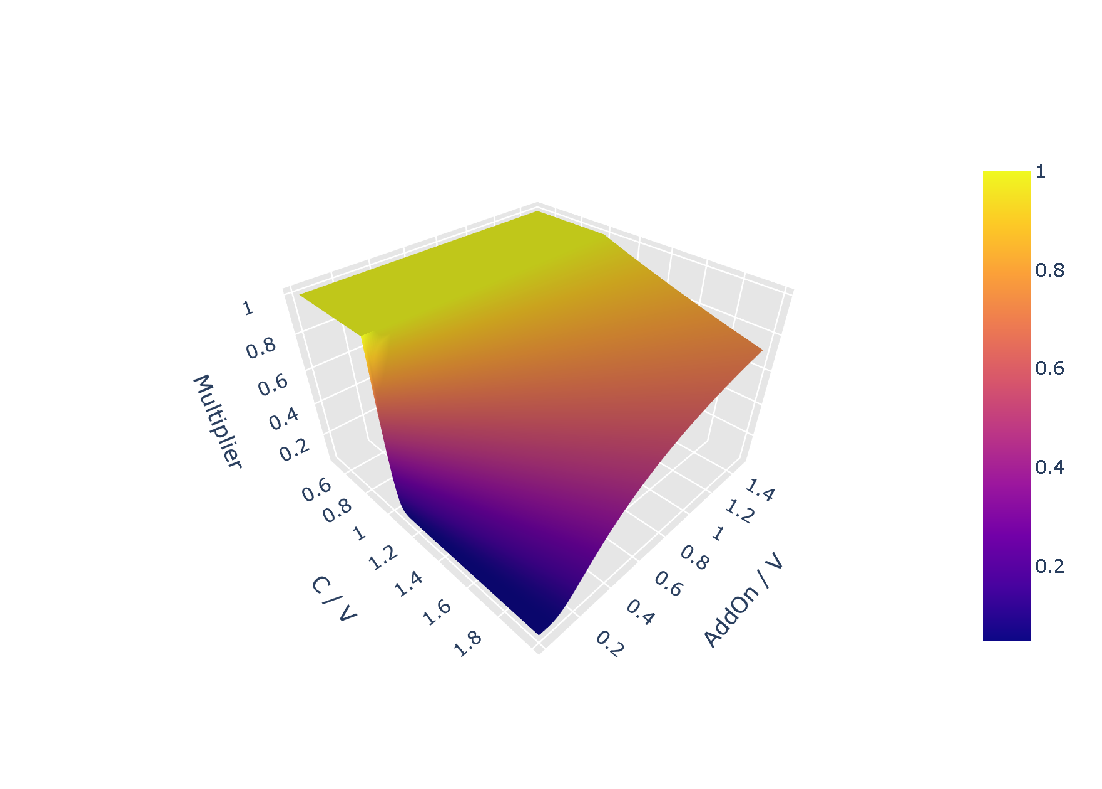
\includegraphics[scale=0.9]{Graphics/SACCR_Multiplier_Function.pdf}
    \caption{}
\end{figure}

    

    
    \hypertarget{addon-calculation}{%
\section{AddOn calculation}\label{addon-calculation}}

Most of the SA-CCR logic is hidden inside the AddOn calculation. At
first it is important to define the following four data parameters:

\hypertarget{m_i}{%
\subparagraph{\texorpdfstring{\(M_i\)}{M\_i}}\label{m_i}}

\begin{quote}
Maturity of the derivative contract. If the underlying of a derivative
is another derivative - e.g.~in the case of a swaption the maturity date
of the underlying needs to be chosen.
\end{quote}

\hypertarget{s_i}{%
\subparagraph{\texorpdfstring{\(S_i\)}{S\_i}}\label{s_i}}

\begin{quote}
For interest rate and credit derivatives the start date of the time
periodreferenced by an interst rate or credit contract. If the
derivtives underlying is another interest rate or credit intsrument (eg
swaption or bond option) \(S_i\) is the start date of the underlying
instead.
\end{quote}

\hypertarget{e_i}{%
\subparagraph{\texorpdfstring{\(E_i\)}{E\_i}}\label{e_i}}

\begin{quote}
Defined as \(S_i\) but referencing the end date instead of the start
date.
\end{quote}

\hypertarget{t_i}{%
\subparagraph{\texorpdfstring{\(T_i\)}{T\_i}}\label{t_i}}

\begin{quote}
For options across all asset classes this is the latest contractual
exercise date.
\end{quote}

    \hypertarget{trade-level-adjusted-notional}{%
\subsection{Trade level adjusted
notional}\label{trade-level-adjusted-notional}}

Each trade \(i\) has a trade level adjusted notional \(d_i^a\) assigned
to it. This is calculated differently for the different asset classes.

\hypertarget{interest-rate-and-credit-derivatives}{%
\paragraph{Interest rate and credit
derivatives}\label{interest-rate-and-credit-derivatives}}

The notional of the trade is usually a well defined value in domestic
currency for interest rate and credit derivatives. It is multiplied by a
supervisory duration factor. The basic idea is, that the value of the
derivative can change more the longer the remaining

\begin{align*}
d_i &= \text{Notional}_i * SD_i \\
\\
\text{where} \qquad SD_i &=\frac{\exp\left(-0.05 * S_i\right)-\exp\left(-0.05 * E_i\right)}{0.05}
\end{align*}

\hypertarget{fx-derivatives}{%
\paragraph{FX derivatives}\label{fx-derivatives}}

While the wording in the BCBS paper is a bit more specific we will just
assume that every FX traded derivative has a USD leg and set the
notional equal the to USD notional.

\hypertarget{equity-and-commodity-derivatives}{%
\paragraph{Equity and commodity
derivatives}\label{equity-and-commodity-derivatives}}

The notional is defined as the price of the underlying. Therefore, it
fluctuates over time.

\hypertarget{notional-of-exotic-derivatives}{%
\paragraph{Notional of exotic
derivatives}\label{notional-of-exotic-derivatives}}

For more exotic derivatives which do have adjustable notionals,
resetting notionals etc. detailed handling of the notional is defined in
paragraph 158.

    Within this thesis we investigate only equity and interest rate
derivatives. For these we can make a few exemplary calculations of the
trade level adjusted notional.

For equity trades determining the trade level adjusted notional is
trivial as it always is the spot price of the underlying. As an example
consider the two trades defined below:

    \begin{tcolorbox}[breakable, size=fbox, boxrule=1pt, pad at break*=1mm,colback=cellbackground, colframe=cellborder]
\prompt{In}{incolor}{In}{\boxspacing}
\begin{Verbatim}[commandchars=\\\{\}]
\PY{c+c1}{\PYZsh{}When the strike is not set explicitly an at the money option is created with K = S(t0)}
\PY{n}{eqOption1} \PY{o}{=} \PY{n}{EquityOption}\PY{p}{(}\PY{n}{maturity} \PY{o}{=} \PY{n}{ql}\PY{o}{.}\PY{n}{Period}\PY{p}{(}\PY{l+m+mi}{1}\PY{p}{,} \PY{n}{ql}\PY{o}{.}\PY{n}{Years}\PY{p}{)}\PY{p}{,}
                         \PY{n}{tradeType}\PY{o}{=} \PY{n}{TradeType}\PY{o}{.}\PY{n}{CALL}\PY{p}{,}
                         \PY{n}{tradeDirection}\PY{o}{=} \PY{n}{TradeDirection}\PY{o}{.}\PY{n}{LONG}\PY{p}{,}
                         \PY{n}{underlying}\PY{o}{=} \PY{n}{Stock}\PY{o}{.}\PY{n}{ADS}\PY{p}{)}

\PY{n}{eqOption2} \PY{o}{=} \PY{n}{EquityOption}\PY{p}{(}\PY{n}{maturity} \PY{o}{=} \PY{n}{ql}\PY{o}{.}\PY{n}{Period}\PY{p}{(}\PY{l+m+mi}{1}\PY{p}{,}   \PY{n}{ql}\PY{o}{.}\PY{n}{Years}\PY{p}{)}\PY{p}{,}
                         \PY{n}{tradeType}\PY{o}{=} \PY{n}{TradeType}\PY{o}{.}\PY{n}{PUT}\PY{p}{,}
                         \PY{n}{tradeDirection}\PY{o}{=} \PY{n}{TradeDirection}\PY{o}{.}\PY{n}{SHORT}\PY{p}{,}
                         \PY{n}{underlying}\PY{o}{=} \PY{n}{Stock}\PY{o}{.}\PY{n}{ADS}\PY{p}{,}
                         \PY{n}{strike} \PY{o}{=} \PY{l+m+mi}{60}\PY{p}{)}
\end{Verbatim}
\end{tcolorbox}

    Let the spot price of Adidas stock be 42. Then, the adjusted notional of
\texttt{eqOption1}, an at the money call on Adidas, is 42 and the
adjusted notional of \texttt{eqOption2}, a short in the money put on
Adidas, is also 42.

    
    For interest rate derivatives such as interest rate swaps or swaptions
on the other hand, the notional is adjusted by the supervisory duration
factor. As the supervisory duration depends on \emph{S} and \emph{E} it
is important to understand how these are determined for the different
interest rate derivatives.

\begin{longtable}[]{@{}lll@{}}
\toprule
\begin{minipage}[b]{0.24\columnwidth}\raggedright
Trade Type\strut
\end{minipage} & \begin{minipage}[b]{0.32\columnwidth}\raggedright
\emph{S}\strut
\end{minipage} & \begin{minipage}[b]{0.36\columnwidth}\raggedright
\emph{E}\strut
\end{minipage}\tabularnewline
\midrule
\endhead
\begin{minipage}[t]{0.24\columnwidth}\raggedright
\textbf{Interest Rate Swap}\strut
\end{minipage} & \begin{minipage}[t]{0.32\columnwidth}\raggedright
Current date\strut
\end{minipage} & \begin{minipage}[t]{0.36\columnwidth}\raggedright
Maturity date\strut
\end{minipage}\tabularnewline
\begin{minipage}[t]{0.24\columnwidth}\raggedright
\textbf{Forward starting IRS}\strut
\end{minipage} & \begin{minipage}[t]{0.32\columnwidth}\raggedright
Start date of the underlying swap\strut
\end{minipage} & \begin{minipage}[t]{0.36\columnwidth}\raggedright
Maturity date of the underlying swap\strut
\end{minipage}\tabularnewline
\begin{minipage}[t]{0.24\columnwidth}\raggedright
\textbf{Swaption}\strut
\end{minipage} & \begin{minipage}[t]{0.32\columnwidth}\raggedright
Start date of the underlying swap\strut
\end{minipage} & \begin{minipage}[t]{0.36\columnwidth}\raggedright
Maturity data of the underlying swap\strut
\end{minipage}\tabularnewline
\bottomrule
\end{longtable}

    \hypertarget{supervisory-delta-adjustments-delta_i}{%
\subsection{\texorpdfstring{Supervisory delta adjustments:
\(\delta_i\)}{Supervisory delta adjustments: \textbackslash{}delta\_i}}\label{supervisory-delta-adjustments-delta_i}}

For linear derivatives \(\delta\) is 1 for long derivatives and -1 for
short derivatives.

For options \(\delta\) is defined as under Black-Scholes:

\begin{align*}
\delta_{\text{long Call}} &= +\Phi\left(\frac{\ln\left(P_i / K_i \right) + 0.5 * \sigma_i^2 * T_i}{\sigma_i * \sqrt{T_i}}\right) \\
\\
\text{where} \qquad \Phi &: \text{standard normal cdf} \\
\sigma_i &: \text{supervisory volatility as defined in Table 2 in paragraph 183}
\end{align*}

This delta is multiplied by -1 in case of a long Put option or a short
Call option. This formula is used for both, equity options and
swaptions.

No detail is given at this point on the delta calculation of CDO
tranches as these are not in the scope of this thesis.

    In the case of an european equity option the parametrization is quite
straight forward.

\(\sigma_i\): 1.2 is the supervisory volatility for a single stock
option

\(K_i\): The strike of the option

\(P_i\): The spot price of the underlying stock

\(T_i\): The maturity of the option

A swaption on the other hand is parametrized as follows for calculation
of its supervisory delta:

\(\sigma_i\): 0.5 is the supervisory volatility for any interst rate
option.

\(K_i\): The strike of the option is the fixed rate of the underlying
swap

\(P_i\): Is the current par rate of the underlying (forward starting)
swap

\(T_i\): The maturity of the option. Please note the difference to
\(E_i\) used for calculation of the adjusted notional, which is the
maturity of the underlying swap.

SA-CCR uses the same Black-Scholes based formula for Swaps as it uses
for Equities. It differentiates options in two dimensions. Whether they
are \emph{bought} or \emph{sold} and whether they are \emph{Call} or
\emph{Put} options (Compare paragraph 159).

SA-CCR defines an option as a call option if it rises in value as the
underlying rises in value. A fixed payer swap rises in value as the
underlying interest rate rises in value. Therefore, an option to buy a
fixed payer swap at a predetermined strike also rises in value as the
underlying interest rate rises in value. Therefore, a swaption on a
payer swap is considered a \emph{Call} under SA-CCR, while a swaption on
a receiver swap is considered a \emph{Put}.

    For the at the money option \texttt{eqOption1} that was set up above we
yield a supervisory delta adjustment of 0.7257.

    
    For an examplary short european swaption that has a par swap as
underlying (i.e.~the NPV of the swap is 0) that is set up as follows:

    \begin{tcolorbox}[breakable, size=fbox, boxrule=1pt, pad at break*=1mm,colback=cellbackground, colframe=cellborder]
\prompt{In}{incolor}{In}{\boxspacing}
\begin{Verbatim}[commandchars=\\\{\}]
\PY{n}{swap} \PY{o}{=} \PY{n}{IRS}\PY{p}{(}\PY{n}{notional}\PY{o}{=}\PY{l+m+mi}{100}\PY{p}{,}
           \PY{n}{timeToSwapStart}\PY{o}{=}\PY{n}{ql}\PY{o}{.}\PY{n}{Period}\PY{p}{(}\PY{l+m+mi}{1}\PY{p}{,} \PY{n}{ql}\PY{o}{.}\PY{n}{Years}\PY{p}{)}\PY{p}{,}
           \PY{n}{timeToSwapEnd}\PY{o}{=}\PY{n}{ql}\PY{o}{.}\PY{n}{Period}\PY{p}{(}\PY{l+m+mi}{3}\PY{p}{,} \PY{n}{ql}\PY{o}{.}\PY{n}{Years}\PY{p}{)}\PY{p}{,}
           \PY{n}{swapDirection}\PY{o}{=}\PY{n}{SwapDirection}\PY{o}{.}\PY{n}{PAYER}\PY{p}{,}
           \PY{n}{index}\PY{o}{=}\PY{n}{InterestRateIndex}\PY{o}{.}\PY{n}{EURIBOR6M}
          \PY{p}{)}

\PY{n}{swaption} \PY{o}{=} \PY{n}{Swaption}\PY{p}{(}\PY{n}{underlyingSwap}\PY{o}{=}\PY{n}{swap}\PY{p}{,}
                    \PY{n}{optionMaturity}\PY{o}{=}\PY{n}{ql}\PY{o}{.}\PY{n}{Period}\PY{p}{(}\PY{l+m+mi}{1}\PY{p}{,} \PY{n}{ql}\PY{o}{.}\PY{n}{Years}\PY{p}{)}\PY{p}{,}
                    \PY{n}{tradeDirection}\PY{o}{=}\PY{n}{TradeDirection}\PY{o}{.}\PY{n}{SHORT}\PY{p}{)}

\PY{n}{SA\PYZus{}CCR}\PY{o}{.}\PY{n}{calculate\PYZus{}sa\PYZus{}ccr\PYZus{}delta}\PY{p}{(}\PY{n}{swaption}\PY{p}{)}
\end{Verbatim}
\end{tcolorbox}

            \begin{tcolorbox}[breakable, size=fbox, boxrule=.5pt, pad at break*=1mm, opacityfill=0]
\prompt{Out}{outcolor}{Out}{\boxspacing}
\begin{Verbatim}[commandchars=\\\{\}]
-0.5987063256828626
\end{Verbatim}
\end{tcolorbox}
        
    we yield a regulatory delta of -0.5987.

    
    \hypertarget{risk-horizon}{%
\subsubsection{Risk Horizon}\label{risk-horizon}}

For unmargined transaction the margining factor is

\[MF^{\text{unmargined}}_i = \sqrt{\frac{\min\left(M_i;1\text{ year}\right)}{1\text{ year}}}\]

This factor can be used to scale down a risk weight calibrated for a 1
year horizon to a shorter period.

With margining the margin period of risk (MPOR) is:

\begin{itemize}
\tightlist
\item
  10 business days for small, uncleared OTC portfolios
\item
  5 business days for cleared derivatives
\item
  20 business days for netting sets with more than 5000 transactions
  that are not with a central counterparty
\item
  and doubling this period for portfolios with outstanding disputes
\end{itemize}

The margining factor is then

\[ MF^{\text{margined}}_i = \frac{3}{2}\sqrt{\frac{MPOR_i}{1\text{ year}}} \]

At this point we need to introduce a collateral agreement object. For
simplicities sake we will not differentiate between collateral and
netting sets in this thesis. All trades that are covered by the same
collateral agreement are also admissible for netting with each other.
(Also refer to the introduction of close out netting above). To take
into account the different parameters determining the risk horizon a
couple of parameters are required to create a collateral agreement. As
an example, below we are setting up a collateral agreement for uncleared
derivatives without exchange of variation margin or initial margin.

    \begin{tcolorbox}[breakable, size=fbox, boxrule=1pt, pad at break*=1mm,colback=cellbackground, colframe=cellborder]
\prompt{In}{incolor}{In}{\boxspacing}
\begin{Verbatim}[commandchars=\\\{\}]
\PY{n}{ca} \PY{o}{=} \PY{n}{CollateralAgreement}\PY{p}{(}
        \PY{n}{margining}\PY{o}{=}\PY{n}{Margining}\PY{o}{.}\PY{n}{UNMARGINED}\PY{p}{,}
        \PY{n}{clearing}\PY{o}{=}\PY{n}{Clearing}\PY{o}{.}\PY{n}{UNCLEARED}\PY{p}{,}
        \PY{n}{tradecount}\PY{o}{=}\PY{n}{Tradecount}\PY{o}{.}\PY{n}{UNDER\PYZus{}FIVE\PYZus{}THOUSAND}\PY{p}{,}
        \PY{n}{dispute}\PY{o}{=}\PY{n}{Dispute}\PY{o}{.}\PY{n}{NO\PYZus{}OUTSTANDING\PYZus{}DISPUTES}\PY{p}{,}
        \PY{n}{threshold}\PY{o}{=}\PY{l+m+mf}{0.0}\PY{p}{,}      \PY{c+c1}{\PYZsh{}Threshold to trigger a margin call}
        \PY{n}{mta}\PY{o}{=}\PY{l+m+mf}{0.0}\PY{p}{,}            \PY{c+c1}{\PYZsh{}Minimum transfer amount for a margin call}
        \PY{n}{vm}\PY{o}{=}\PY{l+m+mf}{0.0}\PY{p}{,}             \PY{c+c1}{\PYZsh{}Variation margin balance}
        \PY{n}{posted\PYZus{}im}\PY{o}{=}\PY{l+m+mf}{0.0}\PY{p}{,}      \PY{c+c1}{\PYZsh{}posted initial margin}
        \PY{n}{received\PYZus{}im}\PY{o}{=}\PY{l+m+mf}{0.0}     \PY{c+c1}{\PYZsh{}received initial margin}
        \PY{p}{)}
\end{Verbatim}
\end{tcolorbox}

    The SA\_CCR paper provides a small exemplary portfolio in Annex 4a
Example 1. It consists of the following trades:

\begin{longtable}[]{@{}llllllll@{}}
\toprule
\begin{minipage}[b]{0.04\columnwidth}\raggedright
Trade \#\strut
\end{minipage} & \begin{minipage}[b]{0.10\columnwidth}\raggedright
Nature\strut
\end{minipage} & \begin{minipage}[b]{0.09\columnwidth}\raggedright
Residual Maturity\strut
\end{minipage} & \begin{minipage}[b]{0.07\columnwidth}\raggedright
Base Ccy\strut
\end{minipage} & \begin{minipage}[b]{0.11\columnwidth}\raggedright
Notional (tsd)\strut
\end{minipage} & \begin{minipage}[b]{0.11\columnwidth}\raggedright
Pay Leg\strut
\end{minipage} & \begin{minipage}[b]{0.13\columnwidth}\raggedright
Receive Leg\strut
\end{minipage} & \begin{minipage}[b]{0.13\columnwidth}\raggedright
Market value (tsd)\strut
\end{minipage}\tabularnewline
\midrule
\endhead
\begin{minipage}[t]{0.04\columnwidth}\raggedright
1\strut
\end{minipage} & \begin{minipage}[t]{0.10\columnwidth}\raggedright
Interest rate swap\strut
\end{minipage} & \begin{minipage}[t]{0.09\columnwidth}\raggedright
10 years\strut
\end{minipage} & \begin{minipage}[t]{0.07\columnwidth}\raggedright
USD\strut
\end{minipage} & \begin{minipage}[t]{0.11\columnwidth}\raggedright
10000\strut
\end{minipage} & \begin{minipage}[t]{0.11\columnwidth}\raggedright
Fixed\strut
\end{minipage} & \begin{minipage}[t]{0.13\columnwidth}\raggedright
Floating\strut
\end{minipage} & \begin{minipage}[t]{0.13\columnwidth}\raggedright
30\strut
\end{minipage}\tabularnewline
\begin{minipage}[t]{0.04\columnwidth}\raggedright
2\strut
\end{minipage} & \begin{minipage}[t]{0.10\columnwidth}\raggedright
Interest rate swap\strut
\end{minipage} & \begin{minipage}[t]{0.09\columnwidth}\raggedright
4 years\strut
\end{minipage} & \begin{minipage}[t]{0.07\columnwidth}\raggedright
USD\strut
\end{minipage} & \begin{minipage}[t]{0.11\columnwidth}\raggedright
10000\strut
\end{minipage} & \begin{minipage}[t]{0.11\columnwidth}\raggedright
Floating\strut
\end{minipage} & \begin{minipage}[t]{0.13\columnwidth}\raggedright
Fixed\strut
\end{minipage} & \begin{minipage}[t]{0.13\columnwidth}\raggedright
-20\strut
\end{minipage}\tabularnewline
\begin{minipage}[t]{0.04\columnwidth}\raggedright
3\strut
\end{minipage} & \begin{minipage}[t]{0.10\columnwidth}\raggedright
European Swaption\strut
\end{minipage} & \begin{minipage}[t]{0.09\columnwidth}\raggedright
1 into 10 years\strut
\end{minipage} & \begin{minipage}[t]{0.07\columnwidth}\raggedright
EUR\strut
\end{minipage} & \begin{minipage}[t]{0.11\columnwidth}\raggedright
5000\strut
\end{minipage} & \begin{minipage}[t]{0.11\columnwidth}\raggedright
Floating\strut
\end{minipage} & \begin{minipage}[t]{0.13\columnwidth}\raggedright
Fixed\strut
\end{minipage} & \begin{minipage}[t]{0.13\columnwidth}\raggedright
50\strut
\end{minipage}\tabularnewline
\bottomrule
\end{longtable}

To set up this examplary portfolio we need to find fixed rates for the
swaps and underlying swaps to match the desired market values.

    Through optimization and using the market data of the 10th of May 2019
the fixed rates to match the market values in Example 1 were identified.

    For trade 1 the matching fixed rate is 2.3754\%, for trade 1 it is
2.2108\% and for the underlying swap of trade 3 it is 0.1610\%

    



    

    
    However, the approach of SA-CCR to use the Black-Scholes for interest
rate derivatives does have a significant flaw.

Obviously, \(\ln\left(P_i / K_i \right)\) is not defined, if \(P_i/K_i\)
is negative. This has, however been very commonplace in recent years,
especially for Euro swaptions. One can always set the fixed rate of the
underlying swap and therefore \(K_i\) as a negative value. But based on
the market data of the 10th of May 2019 it is even possible to yield
negative par rates for the underlying swap.

As an example we are plotting the zero and the 6M forward curve for the
EURIBOR 6M index below. When zooming further in, we can see that that
the 6M forward curve crosses 0 on the 15th of November 2021.




\begin{figure}
	\centering
	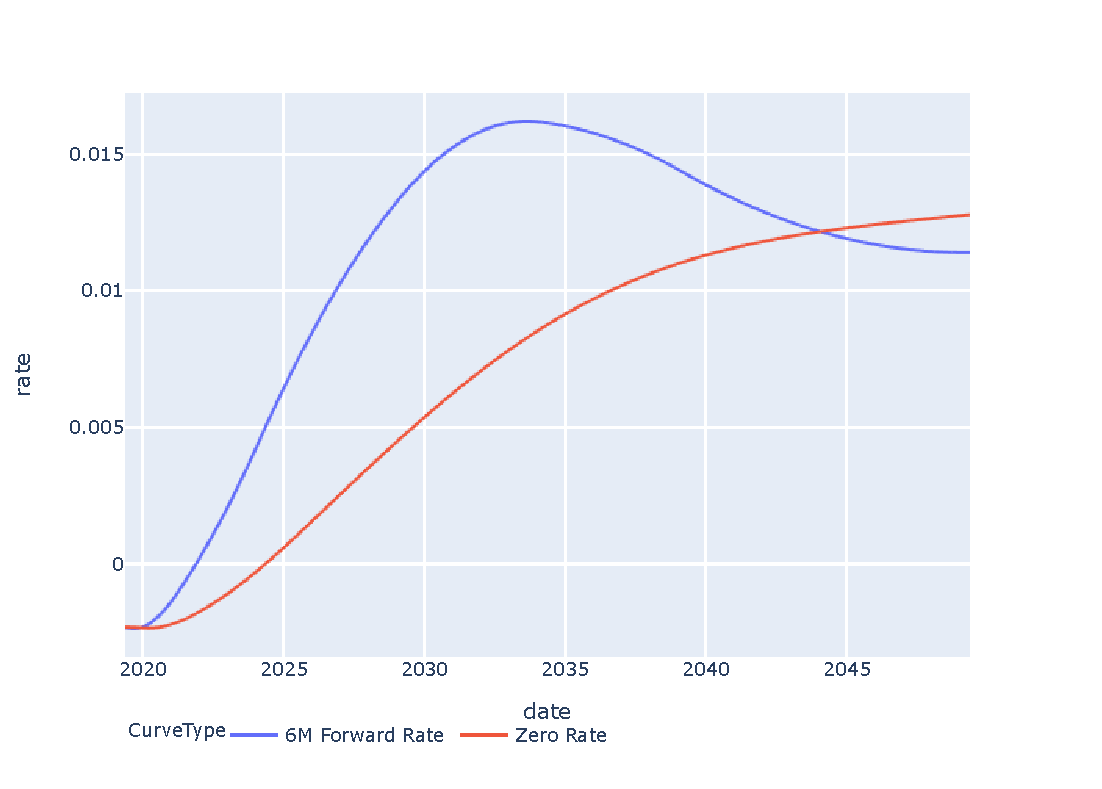
\includegraphics[scale=0.95]{Graphics/euribor6m_termstructure.pdf}
    \caption{}
\end{figure}

\begin{figure}
	\centering
	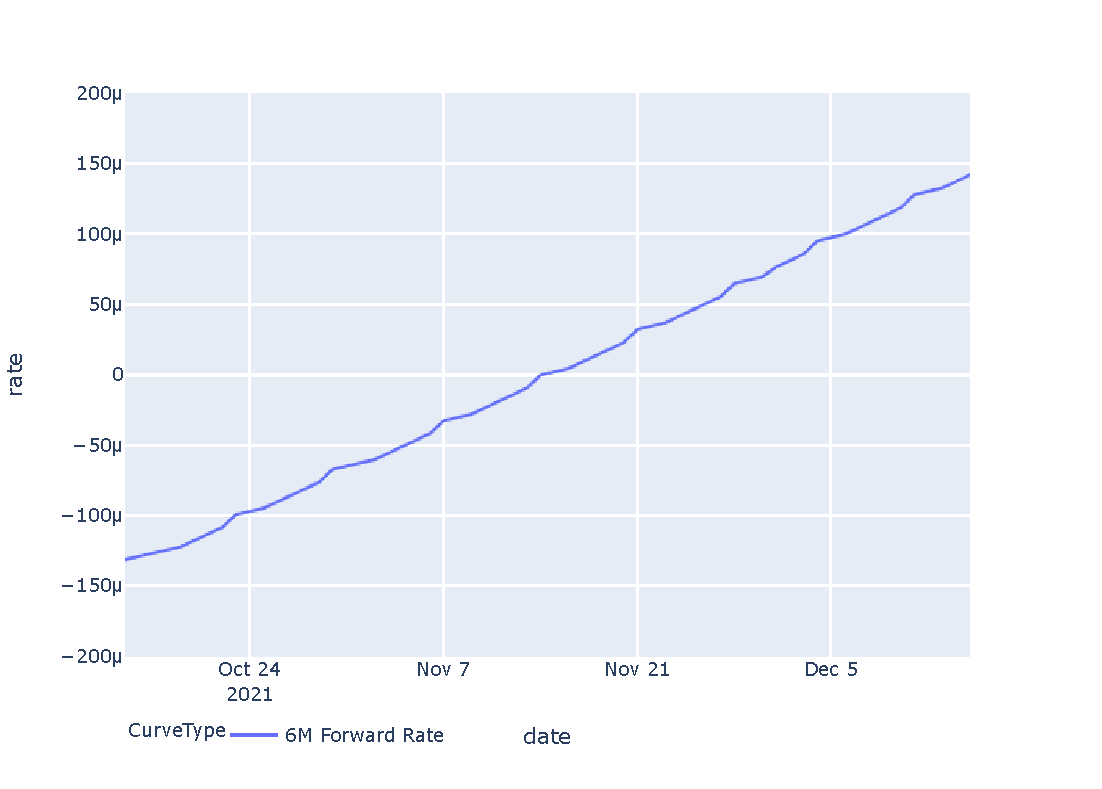
\includegraphics[scale=0.95]{Graphics/euribor6m_termstructure_crossing_zero.pdf}
    \caption{}
\end{figure}

    

    
    To highlight the relationship between the 6M forward curve and the par
rate \(P_i\) of forward starting swap we can set up the following two
swaps depicted below. Since the \(EndDate-StartDate\) for these two
swaps is six months their par rate or fair price can directly be read
from the 6M Forward curve.

    \begin{tcolorbox}[breakable, size=fbox, boxrule=1pt, pad at break*=1mm,colback=cellbackground, colframe=cellborder]
\prompt{In}{incolor}{In}{\boxspacing}
\begin{Verbatim}[commandchars=\\\{\}]
\PY{n+nb}{print}\PY{p}{(}\PY{l+s+s1}{\PYZsq{}}\PY{l+s+s1}{StartDate: }\PY{l+s+s1}{\PYZsq{}} \PY{o}{+} \PY{n+nb}{str}\PY{p}{(}\PY{n}{today}\PY{o}{+}\PY{n}{ql}\PY{o}{.}\PY{n}{Period}\PY{p}{(}\PY{l+m+mi}{30}\PY{p}{,}\PY{n}{ql}\PY{o}{.}\PY{n}{Months}\PY{p}{)}\PY{p}{)}\PY{p}{)}
\PY{n}{swap1} \PY{o}{=} \PY{n}{IRS}\PY{p}{(}\PY{n}{notional}\PY{o}{=}\PY{l+m+mi}{100}\PY{p}{,}
            \PY{n}{timeToSwapStart}\PY{o}{=}\PY{n}{ql}\PY{o}{.}\PY{n}{Period}\PY{p}{(}\PY{l+m+mi}{30}\PY{p}{,}\PY{n}{ql}\PY{o}{.}\PY{n}{Months}\PY{p}{)}\PY{p}{,}
            \PY{n}{timeToSwapEnd}\PY{o}{=}\PY{n}{ql}\PY{o}{.}\PY{n}{Period}\PY{p}{(}\PY{l+m+mi}{36}\PY{p}{,}\PY{n}{ql}\PY{o}{.}\PY{n}{Months}\PY{p}{)}\PY{p}{,}
            \PY{n}{swapDirection}\PY{o}{=}\PY{n}{SwapDirection}\PY{o}{.}\PY{n}{PAYER}\PY{p}{,}
            \PY{n}{index}\PY{o}{=}\PY{n}{InterestRateIndex}\PY{o}{.}\PY{n}{EURIBOR6M}\PY{p}{,}
            \PY{n}{fixed\PYZus{}rate}\PY{o}{=}\PY{l+m+mf}{0.01}
           \PY{p}{)}
\PY{n+nb}{print}\PY{p}{(}\PY{l+s+s1}{\PYZsq{}}\PY{l+s+s1}{ParRate: }\PY{l+s+si}{\PYZpc{}.6f}\PY{l+s+si}{\PYZpc{}\PYZpc{}}\PY{l+s+s1}{\PYZsq{}} \PY{o}{\PYZpc{}} \PY{p}{(}\PY{n}{swap1}\PY{o}{.}\PY{n}{get\PYZus{}par\PYZus{}rate}\PY{p}{(}\PY{p}{)}\PY{o}{*}\PY{l+m+mi}{100}\PY{p}{)}\PY{p}{)}
\end{Verbatim}
\end{tcolorbox}

    \begin{Verbatim}[commandchars=\\\{\}]
StartDate: November 10th, 2021
ParRate: -0.002346\%
    \end{Verbatim}

    \begin{tcolorbox}[breakable, size=fbox, boxrule=1pt, pad at break*=1mm,colback=cellbackground, colframe=cellborder]
\prompt{In}{incolor}{In}{\boxspacing}
\begin{Verbatim}[commandchars=\\\{\}]
\PY{n+nb}{print}\PY{p}{(}\PY{l+s+s1}{\PYZsq{}}\PY{l+s+s1}{StartDate: }\PY{l+s+s1}{\PYZsq{}} \PY{o}{+} \PY{n+nb}{str}\PY{p}{(}\PY{n}{today}\PY{o}{+}\PY{n}{ql}\PY{o}{.}\PY{n}{Period}\PY{p}{(}\PY{l+m+mi}{31}\PY{p}{,}\PY{n}{ql}\PY{o}{.}\PY{n}{Months}\PY{p}{)}\PY{p}{)}\PY{p}{)}
\PY{n}{swap2} \PY{o}{=} \PY{n}{IRS}\PY{p}{(}\PY{n}{notional}\PY{o}{=}\PY{l+m+mi}{100}\PY{p}{,}
            \PY{n}{timeToSwapStart}\PY{o}{=}\PY{n}{ql}\PY{o}{.}\PY{n}{Period}\PY{p}{(}\PY{l+m+mi}{31}\PY{p}{,}\PY{n}{ql}\PY{o}{.}\PY{n}{Months}\PY{p}{)}\PY{p}{,}
            \PY{n}{timeToSwapEnd}\PY{o}{=}\PY{n}{ql}\PY{o}{.}\PY{n}{Period}\PY{p}{(}\PY{l+m+mi}{37}\PY{p}{,} \PY{n}{ql}\PY{o}{.}\PY{n}{Months}\PY{p}{)}\PY{p}{,}
            \PY{n}{swapDirection}\PY{o}{=}\PY{n}{SwapDirection}\PY{o}{.}\PY{n}{PAYER}\PY{p}{,}
            \PY{n}{index}\PY{o}{=}\PY{n}{InterestRateIndex}\PY{o}{.}\PY{n}{EURIBOR6M}\PY{p}{,}
            \PY{n}{fixed\PYZus{}rate}\PY{o}{=}\PY{l+m+mf}{0.01}
            \PY{p}{)}
\PY{n+nb}{print}\PY{p}{(}\PY{l+s+s1}{\PYZsq{}}\PY{l+s+s1}{ParRate: }\PY{l+s+si}{\PYZpc{}.6f}\PY{l+s+si}{\PYZpc{}\PYZpc{}}\PY{l+s+s1}{\PYZsq{}} \PY{o}{\PYZpc{}} \PY{p}{(}\PY{n}{swap2}\PY{o}{.}\PY{n}{get\PYZus{}par\PYZus{}rate}\PY{p}{(}\PY{p}{)}\PY{o}{*}\PY{l+m+mi}{100}\PY{p}{)}\PY{p}{)}
\end{Verbatim}
\end{tcolorbox}

    \begin{Verbatim}[commandchars=\\\{\}]
StartDate: December 10th, 2021
ParRate: 0.011976\%
    \end{Verbatim}




    

    
    \hypertarget{risk-horizon}{%
\subsubsection{Risk Horizon}\label{risk-horizon}}

For unmargined transaction the margining factor is

\[MF^{\text{unmargined}}_i = \sqrt{\frac{\min\left(M_i;1\text{ year}\right)}{1\text{ year}}}\]

This factor can be used to scale down a risk weight calibrated for a 1
year horizon to a shorter period.

With margining the margin period of risk (MPOR) is:

\begin{itemize}
\tightlist
\item
  10 business days for small, uncleared OTC portfolios
\item
  5 business days for cleared derivatives
\item
  20 business days for netting sets with more than 5000 transactions
  that are not with a central counterparty
\item
  and doubling this period for portfolios with outstanding disputes
\end{itemize}

The margining factor is then

\[ MF^{\text{margined}}_i = \frac{3}{2}\sqrt{\frac{MPOR_i}{1\text{ year}}} \]

At this point we need to introduce a collateral agreement object. For
simplicities sake we will not differentiate between collateral and
netting sets in this thesis. All trades that are covered by the same
collateral agreement are also admissible for netting with each other.
(Also refer to the introduction of close out netting above). To take
into account the different parameters determining the risk horizon a
couple of parameters are required to create a collateral agreement. As
an example, below we are setting up a collateral agreement for uncleared
derivatives without exchange of variation margin or initial margin.

    \begin{tcolorbox}[breakable, size=fbox, boxrule=1pt, pad at break*=1mm,colback=cellbackground, colframe=cellborder]
\prompt{In}{incolor}{In}{\boxspacing}
\begin{Verbatim}[commandchars=\\\{\}]
\PY{n}{ca} \PY{o}{=} \PY{n}{CollateralAgreement}\PY{p}{(}
        \PY{n}{margining}\PY{o}{=}\PY{n}{Margining}\PY{o}{.}\PY{n}{UNMARGINED}\PY{p}{,}
        \PY{n}{clearing}\PY{o}{=}\PY{n}{Clearing}\PY{o}{.}\PY{n}{UNCLEARED}\PY{p}{,}
        \PY{n}{tradecount}\PY{o}{=}\PY{n}{Tradecount}\PY{o}{.}\PY{n}{UNDER\PYZus{}FIVE\PYZus{}THOUSAND}\PY{p}{,}
        \PY{n}{dispute}\PY{o}{=}\PY{n}{Dispute}\PY{o}{.}\PY{n}{NO\PYZus{}OUTSTANDING\PYZus{}DISPUTES}\PY{p}{,}
        \PY{n}{threshold}\PY{o}{=}\PY{l+m+mf}{0.0}\PY{p}{,}      \PY{c+c1}{\PYZsh{}Threshold to trigger a margin call}
        \PY{n}{mta}\PY{o}{=}\PY{l+m+mf}{0.0}\PY{p}{,}            \PY{c+c1}{\PYZsh{}Minimum transfer amount for a margin call}
        \PY{n}{vm}\PY{o}{=}\PY{l+m+mf}{0.0}\PY{p}{,}             \PY{c+c1}{\PYZsh{}Variation margin balance}
        \PY{n}{posted\PYZus{}im}\PY{o}{=}\PY{l+m+mf}{0.0}\PY{p}{,}      \PY{c+c1}{\PYZsh{}posted initial margin}
        \PY{n}{received\PYZus{}im}\PY{o}{=}\PY{l+m+mf}{0.0}     \PY{c+c1}{\PYZsh{}received initial margin}
        \PY{p}{)}
\end{Verbatim}
\end{tcolorbox}

    With this collateral set object we can define a function for calculation
the margining factor:

    For trades of differing maturity let's compare the margining factor for
the three most common scenarios:

\begin{enumerate}
\def\labelenumi{\arabic{enumi}.}
\tightlist
\item
  No margining
\item
  Bilateral margining
\item
  Centrally cleared
\end{enumerate}
 
            \begin{tcolorbox}[breakable, size=fbox, boxrule=.5pt, pad at break*=1mm, opacityfill=0]
\prompt{Out}{outcolor}{Out}{}
    
    \centering{\begin{tabular}{lrrrrr}
\toprule
{} &  Three days &  Two weeks &  Six months &  One year &  Ten years \\
\midrule
No margining        &      0.2000 &     0.2000 &      0.7071 &    1.0000 &     1.0000 \\
Bilateral margining &      0.3000 &     0.3000 &      0.3000 &    0.3000 &     0.3000 \\
Centrally cleared   &      0.2121 &     0.2121 &      0.2121 &    0.2121 &     0.2121 \\
\bottomrule
\end{tabular}
}
                \end{tcolorbox}

    




    

    
    \begin{tcolorbox}[breakable, size=fbox, boxrule=1pt, pad at break*=1mm,colback=cellbackground, colframe=cellborder]
\prompt{In}{incolor}{In}{\boxspacing}
\begin{Verbatim}[commandchars=\\\{\}]
\PY{c+c1}{\PYZsh{}import cell}
\PY{k+kn}{import} \PY{n+nn}{QuantLib} \PY{k}{as} \PY{n+nn}{ql}
\PY{k+kn}{from} \PY{n+nn}{IPython}\PY{n+nn}{.}\PY{n+nn}{core}\PY{n+nn}{.}\PY{n+nn}{display} \PY{k+kn}{import} \PY{n}{display}\PY{p}{,} \PY{n}{Markdown}
\PY{k+kn}{from} \PY{n+nn}{scipy} \PY{k+kn}{import} \PY{n}{optimize}
\PY{k+kn}{from} \PY{n+nn}{collateralAgreement} \PY{k+kn}{import} \PY{n}{CollateralAgreement}
\PY{k+kn}{from} \PY{n+nn}{instruments}\PY{n+nn}{.}\PY{n+nn}{interestRateInstrument}\PY{n+nn}{.}\PY{n+nn}{irs} \PY{k+kn}{import} \PY{n}{IRS}
\PY{k+kn}{from} \PY{n+nn}{instruments}\PY{n+nn}{.}\PY{n+nn}{interestRateInstrument}\PY{n+nn}{.}\PY{n+nn}{swaption} \PY{k+kn}{import} \PY{n}{Swaption}
\PY{k+kn}{from} \PY{n+nn}{jupyterUtils} \PY{k+kn}{import} \PY{n}{export}
\PY{k+kn}{from} \PY{n+nn}{marketdata}\PY{n+nn}{.}\PY{n+nn}{fx\PYZus{}spot} \PY{k+kn}{import} \PY{n}{FxSpot}
\PY{k+kn}{from} \PY{n+nn}{marketdata}\PY{n+nn}{.}\PY{n+nn}{interestRateIndices} \PY{k+kn}{import} \PY{n}{InterestRateIndex}
\PY{k+kn}{from} \PY{n+nn}{sa\PYZus{}ccr}\PY{n+nn}{.}\PY{n+nn}{sa\PYZus{}ccr} \PY{k+kn}{import} \PY{n}{SA\PYZus{}CCR}
\PY{k+kn}{from} \PY{n+nn}{utilities}\PY{n+nn}{.}\PY{n+nn}{Enums} \PY{k+kn}{import} \PY{n}{SwapDirection}\PY{p}{,} \PY{n}{TradeDirection}
\PY{n}{asdf} \PY{o}{=}\PY{l+m+mi}{1}
\end{Verbatim}
\end{tcolorbox}

    \hypertarget{addon-for-interest-rate-derivatives}{%
\subsection{AddOn for interest rate
derivatives}\label{addon-for-interest-rate-derivatives}}

\hypertarget{step-1---calculation-of-effective-notional-d_jkir}{%
\paragraph{\texorpdfstring{Step 1 - calculation of effective notional
\(D_{jk}^{IR}\)}{Step 1 - calculation of effective notional D\_\{jk\}\^{}\{IR\}}}\label{step-1---calculation-of-effective-notional-d_jkir}}

\begin{align*}
D_{jk}^{IR} &= \sum_{i\in\left\{Ccy_j, MB_k\right\}}{\delta_i*d_i^{IR}*MF_i}
\end{align*}

Here, the notation \(i\in\left\{Ccy_j, MB_k\right\}\) refers to trades
whose underlying is the interest rate of a common currency \(j\) and
which mature in a common maturity bucket \(k\)

    We can test our implementation of the effective notional against a small
exemplary portfolio in Annex 4a Example 1 of the SA\_CCR paper. It
consists of the following trades:

\begin{longtable}[]{@{}llllllll@{}}
\toprule
\begin{minipage}[b]{0.04\columnwidth}\raggedright
Trade \#\strut
\end{minipage} & \begin{minipage}[b]{0.10\columnwidth}\raggedright
Nature\strut
\end{minipage} & \begin{minipage}[b]{0.09\columnwidth}\raggedright
Residual Maturity\strut
\end{minipage} & \begin{minipage}[b]{0.07\columnwidth}\raggedright
Base Ccy\strut
\end{minipage} & \begin{minipage}[b]{0.11\columnwidth}\raggedright
Notional (tsd)\strut
\end{minipage} & \begin{minipage}[b]{0.11\columnwidth}\raggedright
Pay Leg\strut
\end{minipage} & \begin{minipage}[b]{0.13\columnwidth}\raggedright
Receive Leg\strut
\end{minipage} & \begin{minipage}[b]{0.13\columnwidth}\raggedright
Market value (tsd)\strut
\end{minipage}\tabularnewline
\midrule
\endhead
\begin{minipage}[t]{0.04\columnwidth}\raggedright
1\strut
\end{minipage} & \begin{minipage}[t]{0.10\columnwidth}\raggedright
Interest rate swap\strut
\end{minipage} & \begin{minipage}[t]{0.09\columnwidth}\raggedright
10 years\strut
\end{minipage} & \begin{minipage}[t]{0.07\columnwidth}\raggedright
USD\strut
\end{minipage} & \begin{minipage}[t]{0.11\columnwidth}\raggedright
10000\strut
\end{minipage} & \begin{minipage}[t]{0.11\columnwidth}\raggedright
Fixed\strut
\end{minipage} & \begin{minipage}[t]{0.13\columnwidth}\raggedright
Floating\strut
\end{minipage} & \begin{minipage}[t]{0.13\columnwidth}\raggedright
30\strut
\end{minipage}\tabularnewline
\begin{minipage}[t]{0.04\columnwidth}\raggedright
2\strut
\end{minipage} & \begin{minipage}[t]{0.10\columnwidth}\raggedright
Interest rate swap\strut
\end{minipage} & \begin{minipage}[t]{0.09\columnwidth}\raggedright
4 years\strut
\end{minipage} & \begin{minipage}[t]{0.07\columnwidth}\raggedright
USD\strut
\end{minipage} & \begin{minipage}[t]{0.11\columnwidth}\raggedright
10000\strut
\end{minipage} & \begin{minipage}[t]{0.11\columnwidth}\raggedright
Floating\strut
\end{minipage} & \begin{minipage}[t]{0.13\columnwidth}\raggedright
Fixed\strut
\end{minipage} & \begin{minipage}[t]{0.13\columnwidth}\raggedright
-20\strut
\end{minipage}\tabularnewline
\begin{minipage}[t]{0.04\columnwidth}\raggedright
3\strut
\end{minipage} & \begin{minipage}[t]{0.10\columnwidth}\raggedright
European Swaption\strut
\end{minipage} & \begin{minipage}[t]{0.09\columnwidth}\raggedright
1 into 10 years\strut
\end{minipage} & \begin{minipage}[t]{0.07\columnwidth}\raggedright
EUR\strut
\end{minipage} & \begin{minipage}[t]{0.11\columnwidth}\raggedright
5000\strut
\end{minipage} & \begin{minipage}[t]{0.11\columnwidth}\raggedright
Floating\strut
\end{minipage} & \begin{minipage}[t]{0.13\columnwidth}\raggedright
Fixed\strut
\end{minipage} & \begin{minipage}[t]{0.13\columnwidth}\raggedright
50\strut
\end{minipage}\tabularnewline
\bottomrule
\end{longtable}

To set up this exemplary portfolio we need to find fixed rates for the
swaps and underlying swaps to match the desired market values.

    \begin{tcolorbox}[breakable, size=fbox, boxrule=1pt, pad at break*=1mm,colback=cellbackground, colframe=cellborder]
\prompt{In}{incolor}{In}{\boxspacing}
\begin{Verbatim}[commandchars=\\\{\}]
\PY{k}{def} \PY{n+nf}{find\PYZus{}1}\PY{p}{(}\PY{n}{fixed\PYZus{}rate}\PY{p}{)}\PY{p}{:}
    \PY{n}{target\PYZus{}value} \PY{o}{=} \PY{l+m+mi}{30000}
    \PY{n}{swap} \PY{o}{=} \PY{n}{IRS}\PY{p}{(}\PY{n}{notional} \PY{o}{=} \PY{l+m+mi}{10000000}\PY{p}{,}
               \PY{n}{timeToSwapStart}\PY{o}{=}\PY{n}{ql}\PY{o}{.}\PY{n}{Period}\PY{p}{(}\PY{l+m+mi}{2}\PY{p}{,} \PY{n}{ql}\PY{o}{.}\PY{n}{Days}\PY{p}{)}\PY{p}{,}
               \PY{n}{timeToSwapEnd}\PY{o}{=}\PY{n}{ql}\PY{o}{.}\PY{n}{Period}\PY{p}{(}\PY{l+m+mi}{10}\PY{p}{,} \PY{n}{ql}\PY{o}{.}\PY{n}{Years}\PY{p}{)}\PY{p}{,}
               \PY{n}{swapDirection}\PY{o}{=}\PY{n}{SwapDirection}\PY{o}{.}\PY{n}{PAYER}\PY{p}{,}
               \PY{n}{index} \PY{o}{=} \PY{n}{InterestRateIndex}\PY{o}{.}\PY{n}{USDLIBOR3M}\PY{p}{,}
               \PY{n}{fixed\PYZus{}rate}\PY{o}{=}\PY{n}{fixed\PYZus{}rate}\PY{p}{[}\PY{l+m+mi}{0}\PY{p}{]}
               \PY{p}{)}
    \PY{k}{return} \PY{n+nb}{abs}\PY{p}{(}\PY{n}{swap}\PY{o}{.}\PY{n}{get\PYZus{}price}\PY{p}{(}\PY{p}{)}\PY{o}{\PYZhy{}}\PY{n}{target\PYZus{}value}\PY{p}{)}

\PY{k}{def} \PY{n+nf}{find\PYZus{}2}\PY{p}{(}\PY{n}{fixed\PYZus{}rate}\PY{p}{)}\PY{p}{:}
    \PY{n}{target\PYZus{}value} \PY{o}{=} \PY{o}{\PYZhy{}}\PY{l+m+mi}{20000}
    \PY{n}{swap} \PY{o}{=} \PY{n}{IRS}\PY{p}{(}\PY{n}{notional} \PY{o}{=} \PY{l+m+mi}{10000000}\PY{p}{,}
               \PY{n}{timeToSwapStart}\PY{o}{=}\PY{n}{ql}\PY{o}{.}\PY{n}{Period}\PY{p}{(}\PY{l+m+mi}{2}\PY{p}{,} \PY{n}{ql}\PY{o}{.}\PY{n}{Days}\PY{p}{)}\PY{p}{,}
               \PY{n}{timeToSwapEnd}\PY{o}{=}\PY{n}{ql}\PY{o}{.}\PY{n}{Period}\PY{p}{(}\PY{l+m+mi}{4}\PY{p}{,} \PY{n}{ql}\PY{o}{.}\PY{n}{Years}\PY{p}{)}\PY{p}{,}
               \PY{n}{swapDirection}\PY{o}{=}\PY{n}{SwapDirection}\PY{o}{.}\PY{n}{RECEIVER}\PY{p}{,}
               \PY{n}{index} \PY{o}{=} \PY{n}{InterestRateIndex}\PY{o}{.}\PY{n}{USDLIBOR3M}\PY{p}{,}
               \PY{n}{fixed\PYZus{}rate}\PY{o}{=}\PY{n}{fixed\PYZus{}rate}\PY{p}{[}\PY{l+m+mi}{0}\PY{p}{]}
               \PY{p}{)}
    \PY{k}{return} \PY{n+nb}{abs}\PY{p}{(}\PY{n}{swap}\PY{o}{.}\PY{n}{get\PYZus{}price}\PY{p}{(}\PY{p}{)}\PY{o}{\PYZhy{}}\PY{n}{target\PYZus{}value}\PY{p}{)}

\PY{k}{def} \PY{n+nf}{find\PYZus{}3}\PY{p}{(}\PY{n}{fixed\PYZus{}rate}\PY{p}{)}\PY{p}{:}
    \PY{n}{target\PYZus{}value} \PY{o}{=} \PY{l+m+mi}{50000}
    \PY{n}{notional} \PY{o}{=} \PY{l+m+mi}{5000000}\PY{o}{*}\PY{n}{FxSpot}\PY{o}{.}\PY{n}{USDEUR}\PY{o}{.}\PY{n}{value}
    \PY{n}{swap} \PY{o}{=} \PY{n}{IRS}\PY{p}{(}\PY{n}{notional} \PY{o}{=} \PY{n}{notional}\PY{p}{,}
               \PY{n}{timeToSwapStart}\PY{o}{=}\PY{n}{ql}\PY{o}{.}\PY{n}{Period}\PY{p}{(}\PY{l+m+mi}{1}\PY{p}{,} \PY{n}{ql}\PY{o}{.}\PY{n}{Years}\PY{p}{)}\PY{p}{,}
               \PY{n}{timeToSwapEnd}\PY{o}{=}\PY{n}{ql}\PY{o}{.}\PY{n}{Period}\PY{p}{(}\PY{l+m+mi}{10}\PY{p}{,} \PY{n}{ql}\PY{o}{.}\PY{n}{Years}\PY{p}{)}\PY{p}{,}
               \PY{n}{swapDirection}\PY{o}{=}\PY{n}{SwapDirection}\PY{o}{.}\PY{n}{RECEIVER}\PY{p}{,}
               \PY{n}{index} \PY{o}{=} \PY{n}{InterestRateIndex}\PY{o}{.}\PY{n}{EURIBOR6M}\PY{p}{,}
               \PY{n}{fixed\PYZus{}rate}\PY{o}{=}\PY{n}{fixed\PYZus{}rate}\PY{p}{[}\PY{l+m+mi}{0}\PY{p}{]}
               \PY{p}{)}
    \PY{n}{swaption} \PY{o}{=} \PY{n}{Swaption}\PY{p}{(}\PY{n}{underlyingSwap}\PY{o}{=}\PY{n}{swap}\PY{p}{,}
                        \PY{n}{optionMaturity}\PY{o}{=}\PY{n}{ql}\PY{o}{.}\PY{n}{Period}\PY{p}{(}\PY{l+m+mi}{1}\PY{p}{,} \PY{n}{ql}\PY{o}{.}\PY{n}{Years}\PY{p}{)}\PY{p}{,}
                        \PY{n}{tradeDirection}\PY{o}{=}\PY{n}{TradeDirection}\PY{o}{.}\PY{n}{LONG}\PY{p}{)}
    \PY{n}{price} \PY{o}{=} \PY{n}{swaption}\PY{o}{.}\PY{n}{get\PYZus{}price}\PY{p}{(}\PY{p}{)}\PY{o}{*}\PY{n}{FxSpot}\PY{o}{.}\PY{n}{EURUSD}\PY{o}{.}\PY{n}{value}
    \PY{k}{return} \PY{n+nb}{abs}\PY{p}{(}\PY{n}{price}\PY{o}{\PYZhy{}}\PY{n}{target\PYZus{}value}\PY{p}{)}

\PY{k}{def} \PY{n+nf}{find\PYZus{}4}\PY{p}{(}\PY{n}{fixed\PYZus{}rate}\PY{p}{)}\PY{p}{:}
    \PY{n}{target\PYZus{}value} \PY{o}{=} \PY{o}{\PYZhy{}}\PY{l+m+mf}{0.27}
    \PY{n}{notional} \PY{o}{=} \PY{l+m+mi}{5000000}\PY{o}{*}\PY{n}{FxSpot}\PY{o}{.}\PY{n}{USDEUR}\PY{o}{.}\PY{n}{value}
    \PY{n}{swap} \PY{o}{=} \PY{n}{IRS}\PY{p}{(}\PY{n}{notional} \PY{o}{=} \PY{n}{notional}\PY{p}{,}
               \PY{n}{timeToSwapStart}\PY{o}{=}\PY{n}{ql}\PY{o}{.}\PY{n}{Period}\PY{p}{(}\PY{l+m+mi}{1}\PY{p}{,} \PY{n}{ql}\PY{o}{.}\PY{n}{Years}\PY{p}{)}\PY{p}{,}
               \PY{n}{timeToSwapEnd}\PY{o}{=}\PY{n}{ql}\PY{o}{.}\PY{n}{Period}\PY{p}{(}\PY{l+m+mi}{10}\PY{p}{,} \PY{n}{ql}\PY{o}{.}\PY{n}{Years}\PY{p}{)}\PY{p}{,}
               \PY{n}{swapDirection}\PY{o}{=}\PY{n}{SwapDirection}\PY{o}{.}\PY{n}{RECEIVER}\PY{p}{,}
               \PY{n}{index} \PY{o}{=} \PY{n}{InterestRateIndex}\PY{o}{.}\PY{n}{EURIBOR6M}\PY{p}{,}
               \PY{n}{fixed\PYZus{}rate}\PY{o}{=}\PY{n}{fixed\PYZus{}rate}\PY{p}{[}\PY{l+m+mi}{0}\PY{p}{]}
               \PY{p}{)}
    \PY{n}{swaption} \PY{o}{=} \PY{n}{Swaption}\PY{p}{(}\PY{n}{underlyingSwap}\PY{o}{=}\PY{n}{swap}\PY{p}{,}
                        \PY{n}{optionMaturity}\PY{o}{=}\PY{n}{ql}\PY{o}{.}\PY{n}{Period}\PY{p}{(}\PY{l+m+mi}{1}\PY{p}{,} \PY{n}{ql}\PY{o}{.}\PY{n}{Years}\PY{p}{)}\PY{p}{,}
                        \PY{n}{tradeDirection}\PY{o}{=}\PY{n}{TradeDirection}\PY{o}{.}\PY{n}{LONG}\PY{p}{)}
    \PY{n}{delta} \PY{o}{=} \PY{n}{SA\PYZus{}CCR}\PY{o}{.}\PY{n}{calculate\PYZus{}sa\PYZus{}ccr\PYZus{}delta}\PY{p}{(}\PY{n}{swaption}\PY{p}{)}
    \PY{k}{return} \PY{n+nb}{abs}\PY{p}{(}\PY{n}{delta}\PY{o}{\PYZhy{}}\PY{n}{target\PYZus{}value}\PY{p}{)}

\PY{n}{result} \PY{o}{=} \PY{n}{optimize}\PY{o}{.}\PY{n}{minimize}\PY{p}{(}\PY{n}{find\PYZus{}1}\PY{p}{,} \PY{n}{x0}\PY{o}{=}\PY{l+m+mf}{0.01}\PY{p}{,} \PY{n}{tol}\PY{o}{=}\PY{l+m+mf}{0.0000000001}\PY{p}{)}
\PY{n}{fixed\PYZus{}rate\PYZus{}trade\PYZus{}1} \PY{o}{=} \PY{n}{result}\PY{o}{.}\PY{n}{x}\PY{p}{[}\PY{l+m+mi}{0}\PY{p}{]}
\PY{n}{result} \PY{o}{=} \PY{n}{optimize}\PY{o}{.}\PY{n}{minimize}\PY{p}{(}\PY{n}{find\PYZus{}2}\PY{p}{,} \PY{n}{x0}\PY{o}{=}\PY{l+m+mf}{0.01}\PY{p}{,} \PY{n}{tol}\PY{o}{=}\PY{l+m+mf}{0.0000000001}\PY{p}{)}
\PY{n}{fixed\PYZus{}rate\PYZus{}trade\PYZus{}2} \PY{o}{=} \PY{n}{result}\PY{o}{.}\PY{n}{x}\PY{p}{[}\PY{l+m+mi}{0}\PY{p}{]}
\PY{n}{result} \PY{o}{=} \PY{n}{optimize}\PY{o}{.}\PY{n}{minimize}\PY{p}{(}\PY{n}{find\PYZus{}3}\PY{p}{,} \PY{n}{x0}\PY{o}{=}\PY{l+m+mf}{0.01}\PY{p}{,} \PY{n}{constraints}\PY{o}{=}\PY{p}{\PYZob{}}\PY{l+s+s1}{\PYZsq{}}\PY{l+s+s1}{type}\PY{l+s+s1}{\PYZsq{}}\PY{p}{:}\PY{l+s+s1}{\PYZsq{}}\PY{l+s+s1}{ineq}\PY{l+s+s1}{\PYZsq{}}\PY{p}{,}\PY{l+s+s1}{\PYZsq{}}\PY{l+s+s1}{fun}\PY{l+s+s1}{\PYZsq{}}\PY{p}{:} \PY{k}{lambda} \PY{n}{x}\PY{p}{:} \PY{n}{x}\PY{p}{[}\PY{l+m+mi}{0}\PY{p}{]}\PY{o}{+}\PY{l+m+mf}{0.02}\PY{p}{\PYZcb{}}\PY{p}{,} \PY{n}{tol}\PY{o}{=}\PY{l+m+mf}{0.0000000001}\PY{p}{)}
\PY{n}{fixed\PYZus{}rate\PYZus{}trade\PYZus{}3} \PY{o}{=} \PY{n}{result}\PY{o}{.}\PY{n}{x}\PY{p}{[}\PY{l+m+mi}{0}\PY{p}{]}
\PY{n}{result} \PY{o}{=} \PY{n}{optimize}\PY{o}{.}\PY{n}{minimize}\PY{p}{(}\PY{n}{find\PYZus{}4}\PY{p}{,} \PY{n}{x0}\PY{o}{=}\PY{l+m+mf}{0.01}\PY{p}{,} \PY{n}{constraints}\PY{o}{=}\PY{p}{\PYZob{}}\PY{l+s+s1}{\PYZsq{}}\PY{l+s+s1}{type}\PY{l+s+s1}{\PYZsq{}}\PY{p}{:}\PY{l+s+s1}{\PYZsq{}}\PY{l+s+s1}{ineq}\PY{l+s+s1}{\PYZsq{}}\PY{p}{,}\PY{l+s+s1}{\PYZsq{}}\PY{l+s+s1}{fun}\PY{l+s+s1}{\PYZsq{}}\PY{p}{:} \PY{k}{lambda} \PY{n}{x}\PY{p}{:} \PY{n}{x}\PY{p}{[}\PY{l+m+mi}{0}\PY{p}{]}\PY{p}{\PYZcb{}}\PY{p}{,} \PY{n}{tol}\PY{o}{=}\PY{l+m+mf}{0.0000000001}\PY{p}{)}
\PY{n}{fixed\PYZus{}rate\PYZus{}trade\PYZus{}4} \PY{o}{=} \PY{n}{result}\PY{o}{.}\PY{n}{x}\PY{p}{[}\PY{l+m+mi}{0}\PY{p}{]}
\end{Verbatim}
\end{tcolorbox}

    Through optimization and using the market data of the 10th of May 2019
the fixed rates to match the market values in Example 1 were identified.

    \begin{tcolorbox}[breakable, size=fbox, boxrule=1pt, pad at break*=1mm,colback=cellbackground, colframe=cellborder]
\prompt{In}{incolor}{In}{\boxspacing}
\begin{Verbatim}[commandchars=\\\{\}]
\PY{n}{trade\PYZus{}1} \PY{o}{=} \PY{n}{IRS}\PY{p}{(}\PY{n}{notional} \PY{o}{=} \PY{l+m+mi}{10000000}\PY{p}{,}
             \PY{n}{timeToSwapStart}\PY{o}{=}\PY{n}{ql}\PY{o}{.}\PY{n}{Period}\PY{p}{(}\PY{l+m+mi}{2}\PY{p}{,} \PY{n}{ql}\PY{o}{.}\PY{n}{Days}\PY{p}{)}\PY{p}{,}
             \PY{n}{timeToSwapEnd}\PY{o}{=}\PY{n}{ql}\PY{o}{.}\PY{n}{Period}\PY{p}{(}\PY{l+m+mi}{10}\PY{p}{,} \PY{n}{ql}\PY{o}{.}\PY{n}{Years}\PY{p}{)}\PY{p}{,}
             \PY{n}{swapDirection}\PY{o}{=}\PY{n}{SwapDirection}\PY{o}{.}\PY{n}{PAYER}\PY{p}{,}
             \PY{n}{index} \PY{o}{=} \PY{n}{InterestRateIndex}\PY{o}{.}\PY{n}{USDLIBOR3M}\PY{p}{,}
             \PY{n}{fixed\PYZus{}rate}\PY{o}{=}\PY{n}{fixed\PYZus{}rate\PYZus{}trade\PYZus{}1}
             \PY{p}{)}

\PY{n}{trade\PYZus{}2} \PY{o}{=} \PY{n}{IRS}\PY{p}{(}\PY{n}{notional} \PY{o}{=} \PY{l+m+mi}{10000000}\PY{p}{,}
              \PY{n}{timeToSwapStart}\PY{o}{=}\PY{n}{ql}\PY{o}{.}\PY{n}{Period}\PY{p}{(}\PY{l+m+mi}{2}\PY{p}{,} \PY{n}{ql}\PY{o}{.}\PY{n}{Days}\PY{p}{)}\PY{p}{,}
              \PY{n}{timeToSwapEnd}\PY{o}{=}\PY{n}{ql}\PY{o}{.}\PY{n}{Period}\PY{p}{(}\PY{l+m+mi}{4}\PY{p}{,} \PY{n}{ql}\PY{o}{.}\PY{n}{Years}\PY{p}{)}\PY{p}{,}
              \PY{n}{swapDirection}\PY{o}{=}\PY{n}{SwapDirection}\PY{o}{.}\PY{n}{RECEIVER}\PY{p}{,}
              \PY{n}{index} \PY{o}{=} \PY{n}{InterestRateIndex}\PY{o}{.}\PY{n}{USDLIBOR3M}\PY{p}{,}
              \PY{n}{fixed\PYZus{}rate}\PY{o}{=}\PY{n}{fixed\PYZus{}rate\PYZus{}trade\PYZus{}2}
              \PY{p}{)}

\PY{n}{notional} \PY{o}{=} \PY{l+m+mi}{5000000}\PY{o}{*}\PY{n}{FxSpot}\PY{o}{.}\PY{n}{USDEUR}\PY{o}{.}\PY{n}{value}
\PY{n}{ul\PYZus{}swap} \PY{o}{=} \PY{n}{IRS}\PY{p}{(}\PY{n}{notional} \PY{o}{=} \PY{n}{notional}\PY{p}{,}
              \PY{n}{timeToSwapStart}\PY{o}{=}\PY{n}{ql}\PY{o}{.}\PY{n}{Period}\PY{p}{(}\PY{l+m+mi}{1}\PY{p}{,} \PY{n}{ql}\PY{o}{.}\PY{n}{Years}\PY{p}{)}\PY{p}{,}
              \PY{n}{timeToSwapEnd}\PY{o}{=}\PY{n}{ql}\PY{o}{.}\PY{n}{Period}\PY{p}{(}\PY{l+m+mi}{10}\PY{p}{,} \PY{n}{ql}\PY{o}{.}\PY{n}{Years}\PY{p}{)}\PY{p}{,}
              \PY{n}{swapDirection}\PY{o}{=}\PY{n}{SwapDirection}\PY{o}{.}\PY{n}{RECEIVER}\PY{p}{,}
              \PY{n}{index} \PY{o}{=} \PY{n}{InterestRateIndex}\PY{o}{.}\PY{n}{EURIBOR6M}\PY{p}{,}
              \PY{n}{fixed\PYZus{}rate}\PY{o}{=}\PY{n}{fixed\PYZus{}rate\PYZus{}trade\PYZus{}3}
              \PY{p}{)}

\PY{n}{trade\PYZus{}3} \PY{o}{=} \PY{n}{Swaption}\PY{p}{(}\PY{n}{underlyingSwap}\PY{o}{=}\PY{n}{ul\PYZus{}swap}\PY{p}{,}
                   \PY{n}{optionMaturity}\PY{o}{=}\PY{n}{ql}\PY{o}{.}\PY{n}{Period}\PY{p}{(}\PY{l+m+mi}{1}\PY{p}{,} \PY{n}{ql}\PY{o}{.}\PY{n}{Years}\PY{p}{)}\PY{p}{,}
                   \PY{n}{tradeDirection}\PY{o}{=}\PY{n}{TradeDirection}\PY{o}{.}\PY{n}{LONG}\PY{p}{)}

\PY{n}{test\PYZus{}portfolio} \PY{o}{=} \PY{p}{[}\PY{n}{trade\PYZus{}1}\PY{p}{,} \PY{n}{trade\PYZus{}2}\PY{p}{,} \PY{n}{trade\PYZus{}3}\PY{p}{]}
\end{Verbatim}
\end{tcolorbox}

    \begin{tcolorbox}[breakable, size=fbox, boxrule=1pt, pad at break*=1mm,colback=cellbackground, colframe=cellborder]
\prompt{In}{incolor}{In}{\boxspacing}
\begin{Verbatim}[commandchars=\\\{\}]
\PY{n}{display}\PY{p}{(}\PY{n}{Markdown}\PY{p}{(}\PY{l+s+s1}{\PYZsq{}}\PY{l+s+s1}{For trade 1 the matching fixed rate is }\PY{l+s+si}{\PYZpc{}.4f}\PY{l+s+si}{\PYZpc{}\PYZpc{}}\PY{l+s+s1}{, for trade 1 it is }\PY{l+s+si}{\PYZpc{}.4f}\PY{l+s+si}{\PYZpc{}\PYZpc{}}\PY{l+s+s1}{ and for the underlying swap of trade 3 it is }\PY{l+s+si}{\PYZpc{}.4f}\PY{l+s+si}{\PYZpc{}\PYZpc{}}\PY{l+s+s1}{\PYZsq{}} \PY{o}{\PYZpc{}} \PY{p}{(}\PY{p}{(}\PY{n}{fixed\PYZus{}rate\PYZus{}trade\PYZus{}1}\PY{o}{*}\PY{l+m+mi}{100}\PY{p}{)}\PY{p}{,}\PY{p}{(}\PY{n}{fixed\PYZus{}rate\PYZus{}trade\PYZus{}2}\PY{o}{*}\PY{l+m+mi}{100}\PY{p}{)}\PY{p}{,}\PY{p}{(}\PY{n}{fixed\PYZus{}rate\PYZus{}trade\PYZus{}3}\PY{o}{*}\PY{l+m+mi}{100}\PY{p}{)}\PY{p}{)}\PY{p}{)}\PY{p}{)}
\end{Verbatim}
\end{tcolorbox}

    For trade 1 the matching fixed rate is 2.3754\%, for trade 1 it is
2.2108\% and for the underlying swap of trade 3 it is 0.1610\%

    
    \begin{tcolorbox}[breakable, size=fbox, boxrule=1pt, pad at break*=1mm,colback=cellbackground, colframe=cellborder]
\prompt{In}{incolor}{In}{\boxspacing}
\begin{Verbatim}[commandchars=\\\{\}]
\PY{n}{ca}\PY{o}{=}\PY{n}{CollateralAgreement}\PY{p}{(}\PY{p}{)}

\PY{n+nb}{print}\PY{p}{(}\PY{n}{SA\PYZus{}CCR}\PY{o}{.}\PY{n}{calculate\PYZus{}sa\PYZus{}ccr\PYZus{}delta}\PY{p}{(}\PY{n}{trade\PYZus{}1}\PY{p}{)}\PY{p}{)}
\PY{n+nb}{print}\PY{p}{(}\PY{n}{SA\PYZus{}CCR}\PY{o}{.}\PY{n}{trade\PYZus{}level\PYZus{}adjusted\PYZus{}notional}\PY{p}{(}\PY{n}{trade\PYZus{}1}\PY{p}{)}\PY{p}{)}
\PY{n+nb}{print}\PY{p}{(}\PY{n}{SA\PYZus{}CCR}\PY{o}{.}\PY{n}{calculate\PYZus{}sa\PYZus{}ccr\PYZus{}delta}\PY{p}{(}\PY{n}{trade\PYZus{}2}\PY{p}{)}\PY{p}{)}
\PY{n+nb}{print}\PY{p}{(}\PY{n}{SA\PYZus{}CCR}\PY{o}{.}\PY{n}{trade\PYZus{}level\PYZus{}adjusted\PYZus{}notional}\PY{p}{(}\PY{n}{trade\PYZus{}2}\PY{p}{)}\PY{p}{)}
\PY{n+nb}{print}\PY{p}{(}\PY{n}{SA\PYZus{}CCR}\PY{o}{.}\PY{n}{calculate\PYZus{}sa\PYZus{}ccr\PYZus{}delta}\PY{p}{(}\PY{n}{trade\PYZus{}3}\PY{p}{)}\PY{p}{)}
\PY{n+nb}{print}\PY{p}{(}\PY{n}{SA\PYZus{}CCR}\PY{o}{.}\PY{n}{trade\PYZus{}level\PYZus{}adjusted\PYZus{}notional}\PY{p}{(}\PY{n}{trade\PYZus{}3}\PY{p}{)}\PY{p}{)}

\PY{n}{SA\PYZus{}CCR}\PY{o}{.}\PY{n}{interest\PYZus{}rate\PYZus{}addOn}\PY{p}{(}\PY{n}{test\PYZus{}portfolio}\PY{p}{,}\PY{n}{ca}\PY{p}{)}
\end{Verbatim}
\end{tcolorbox}

    \begin{Verbatim}[commandchars=\\\{\}]
1
78638320.21725275
-1
36198301.54418307
-0.00343382383244269
31712286.360503413
    \end{Verbatim}

            \begin{tcolorbox}[breakable, size=fbox, boxrule=.5pt, pad at break*=1mm, opacityfill=0]
\prompt{Out}{outcolor}{Out}{\boxspacing}
\begin{Verbatim}[commandchars=\\\{\}]
296732.72980308026
\end{Verbatim}
\end{tcolorbox}
        
    \begin{tcolorbox}[breakable, size=fbox, boxrule=1pt, pad at break*=1mm,colback=cellbackground, colframe=cellborder]
\prompt{In}{incolor}{In}{\boxspacing}
\begin{Verbatim}[commandchars=\\\{\}]
\PY{n}{export}\PY{p}{(}\PY{l+s+s2}{\PYZdq{}}\PY{l+s+s2}{SA\PYZus{}CCR\PYZus{}ird\PYZus{}addon.ipynb}\PY{l+s+s2}{\PYZdq{}}\PY{p}{)}
\end{Verbatim}
\end{tcolorbox}





\subsection{Approaches to allocation}
With increasing sophistication of risk, own capital and margining models the need for equally sophisticated tools for attributing these measures rises aswell. Allocating the variation margin or the current exposure method (CEM) to individual trades is trivial as these measures may just be calculated for an individual trade and then added up across all trades to obtain the correct aggregate value. For measures which take portfolio effects into account such as a state of the art VaR model, ISDA-SIMM or SA-CCR however, this approach is not possible. The advent of portfolio based models for internal risk measurement in the late 1990s and for regulatory risk measurement in the late 2000s sparked research into how such measures should be reallocated. Gregory \cite[Chapter~10.7]{gregory2015xva} states that three approaches are used in practice: \begin{itemize}
\item Incremental allocation
\item Marginal allocation 
\item Pro rata allocation
\end{itemize}
Additionally \citep{koyluoglu2002risk}
Eigenschaften von Allokationen
\begin{itemize}
\item Nativ additiv
\item Risk sensitivity
\item Unabhaengig von Portfoliozusammensetzung
\item Stable through time
\end{itemize}



\subsubsection{Incremental allocation}
Incremental allocation can only be applied when observing the development of a portfolio through time. Given a pre-existing portfolio $P$ consisting of $n$ trades $t_1$ through $t_n$ and a portfolio-based measure $M$ the incremental contribution of the first and second additional trade may be calculated as:
\begin{align*}
M_{\text{inc},t_{n+1}} & =M\left(t_1\dots t_{n+1}\right)- M\left(t_1\dots t_{n}\right) \\
M_{\text{inc},t_{n+2}} & =M\left(t_1\dots t_{n+2}\right)- M\left(t_1\dots t_{n+1}\right)
%IncM_{t_{n+1}} =M\left(t_1\dots t_{n+1}\right) - M\left(t_1\dots t_{n+1}\right) \\
%IncM_{t_{n+2}} =M\left(t_1\dots \t_{n+2}\right) - M\left(t_1\dots t_{n+1}\right)
\end{align*}
It can be easily seen that this approach yields a natively additive allocation since it forms a telescoping sum\footnote{For brevity in Notation let $M(t_i)$ be equivalent to $M(t_1\dots t_i)$ 
} :
\begin{align*}
M_{\text{inc},t_1}&=M(t_1) \\
M_{\text{inc},t_i}&= M(t_i)-M(t_{i-1}) \\
M_{\text{inc},t_n}&= M(t_n) - M(t_{n-1})\\
\sum_{i=1}^{n}{M_{\text{inc},i}} &= M(t_1)-M(t_1)+\dots+M(t_{n-1})-M(t_{n-1})+M(t_n) = M(t_n)
\end{align*}
The incremental allocation can be calculated as or before a new trade is added to the portfolio. It is a risk sensitive value when it is calculated as it accurately reflect how the additional trade changes the risk measure. If the trade is mitigating risk at the time of its inception according to $M$ its incremental allocation $M_{inc}$ is negative. If it increases the risk its $M_{inc}$ is positive. However, $M_{inc}$ does not adapt over time and is likely to loose its accurate risk depiction as additional trade are added to the portfolio. As a portfolio develops it may well be possible, that a trade for which a negative $M_{inc}$ was calculated at its inception may loose its risk mitigation. Due to this property $M_{inc}$ of a given trade should ideally only be used at or before trade inception. One such use case is the PnL calculation of a new trade to determine the performance of the trading desk or trader which initiated the trade. Another would be to use it prior to an investment decision \cite{tibiletti2001incremental}. It can however not be used to analyse an existing portfolio to e.g. identify trades which drive risk or determine how increases or decreases in a given position would impact the portfolio measure. It also cant be calculated deterministically a posteriori for a portfolio without knowing its composition through time.

In the past, some academic work focussed on approximating the incremental VaR as it requires a recalculation of the VaR for the entire portfolio. An overview of these works and their potential pitfalls may be found in \cite{tibiletti2001incremental}. Since this work will rather focus on marginal than incremental allocation further details may be found in the referred paper. In the empirical analysis the incremental allocation will be calculated exactly.

\subsubsection{Marginal allocation}

    

    
    Next, we are setting up a function to calculate the \(AddOn\) for
derivatives from the FX asset class. The approach is a little simpler
than that for the IR asset class as no differentiaten between time
buckets is necessary. All derivatives on a common currency pair can be
set off against each other.

\begin{align*}
AddOn^{FX} &= \sum_j{AddOn_{HS_j}^{FX}} \\
AddOn^{FX}_{HS_j} &= SF_j^{FX} * | \text{EffectiveNotional}_j^{FX} | \\
\text{EffectiveNotional}_j^{FX} &= \sum_{i \in HS_j}{\delta_i * d_i^{FX} * MF_i^{type}}
\end{align*}

With the hedging sets \(i \in HS\) referencing all derivatives on a
common currency pair.

    In the following example we will create a swap and display its price.

    \begin{tcolorbox}[breakable, size=fbox, boxrule=1pt, pad at break*=1mm,colback=cellbackground, colframe=cellborder]
\prompt{In}{incolor}{2}{\boxspacing}
\begin{Verbatim}[commandchars=\\\{\}]
\PY{c+c1}{\PYZsh{} Creating a swap}


\PY{n}{irs} \PY{o}{=} \PY{n}{IRS}\PY{p}{(}\PY{n}{notional} \PY{o}{=} \PY{l+m+mi}{100}\PY{p}{,}
    \PY{n}{timeToSwapStart}\PY{o}{=}\PY{n}{ql}\PY{o}{.}\PY{n}{Period}\PY{p}{(}\PY{l+m+mi}{2}\PY{p}{,} \PY{n}{ql}\PY{o}{.}\PY{n}{Days}\PY{p}{)}\PY{p}{,}
    \PY{n}{timeToSwapEnd}\PY{o}{=}\PY{n}{ql}\PY{o}{.}\PY{n}{Period}\PY{p}{(}\PY{l+m+mi}{10}\PY{p}{,} \PY{n}{ql}\PY{o}{.}\PY{n}{Years}\PY{p}{)}\PY{p}{,}
    \PY{n}{swapDirection}\PY{o}{=}\PY{n}{SwapDirection}\PY{o}{.}\PY{n}{PAYER}\PY{p}{,}
    \PY{n}{index}\PY{o}{=}\PY{n}{InterestRateIndex}\PY{o}{.}\PY{n}{EURIBOR6M}\PY{p}{,}
    \PY{n}{fixed\PYZus{}rate}\PY{o}{=}\PY{l+m+mf}{0.02}
    \PY{p}{)}

\PY{n}{irs}\PY{o}{.}\PY{n}{get\PYZus{}price}\PY{p}{(}\PY{p}{)}
\end{Verbatim}
\end{tcolorbox}

            \begin{tcolorbox}[breakable, size=fbox, boxrule=.5pt, pad at break*=1mm, opacityfill=0]
\prompt{Out}{outcolor}{2}{\boxspacing}
\begin{Verbatim}[commandchars=\\\{\}]
-15.11727999472697
\end{Verbatim}
\end{tcolorbox}
        
    \begin{tcolorbox}[breakable, size=fbox, boxrule=1pt, pad at break*=1mm,colback=cellbackground, colframe=cellborder]
\prompt{In}{incolor}{3}{\boxspacing}
\begin{Verbatim}[commandchars=\\\{\}]
\PY{c+c1}{\PYZsh{} Let us also create an OIS}

\PY{n}{ois} \PY{o}{=} \PY{n}{OIS}\PY{p}{(}\PY{n}{notional} \PY{o}{=} \PY{l+m+mi}{1000}\PY{p}{,}
          \PY{n}{timeToSwapStart}\PY{o}{=}\PY{n}{ql}\PY{o}{.}\PY{n}{Period}\PY{p}{(}\PY{l+m+mi}{2}\PY{p}{,} \PY{n}{ql}\PY{o}{.}\PY{n}{Days}\PY{p}{)}\PY{p}{,}
          \PY{n}{timeToSwapEnd}\PY{o}{=}\PY{n}{ql}\PY{o}{.}\PY{n}{Period}\PY{p}{(}\PY{l+m+mi}{10}\PY{p}{,} \PY{n}{ql}\PY{o}{.}\PY{n}{Years}\PY{p}{)}\PY{p}{,}
          \PY{n}{swapDirection}\PY{o}{=}\PY{n}{SwapDirection}\PY{o}{.}\PY{n}{PAYER}\PY{p}{,}
          \PY{n}{index}\PY{o}{=}\PY{n}{InterestRateIndex}\PY{o}{.}\PY{n}{FEDFUNDS}\PY{p}{,}
          \PY{n}{fixed\PYZus{}rate}\PY{o}{=}\PY{l+m+mf}{0.04}\PY{p}{)}

\PY{n}{ois}\PY{o}{.}\PY{n}{get\PYZus{}price}\PY{p}{(}\PY{p}{)}
\end{Verbatim}
\end{tcolorbox}

            \begin{tcolorbox}[breakable, size=fbox, boxrule=.5pt, pad at break*=1mm, opacityfill=0]
\prompt{Out}{outcolor}{3}{\boxspacing}
\begin{Verbatim}[commandchars=\\\{\}]
-165.77717223100274
\end{Verbatim}
\end{tcolorbox}
        
    Now we shall have a final example of this glorious integration of
Jupyter and LaTeX. For this I will create an equity swap and print its
price.

Well, I do think that I do need to change a tiny bit here to be honest.

    \begin{tcolorbox}[breakable, size=fbox, boxrule=1pt, pad at break*=1mm,colback=cellbackground, colframe=cellborder]
\prompt{In}{incolor}{5}{\boxspacing}
\begin{Verbatim}[commandchars=\\\{\}]
\PY{n}{eqopt} \PY{o}{=} \PY{n}{EquityOption}\PY{p}{(}\PY{n}{notional} \PY{o}{=} \PY{l+m+mi}{20}\PY{p}{,}
                     \PY{n}{maturity} \PY{o}{=} \PY{n}{ql}\PY{o}{.}\PY{n}{Period}\PY{p}{(}\PY{l+m+mi}{1}\PY{p}{,} \PY{n}{ql}\PY{o}{.}\PY{n}{Years}\PY{p}{)}\PY{p}{,}
                     \PY{n}{tradeType}\PY{o}{=} \PY{n}{TradeType}\PY{o}{.}\PY{n}{PUT}\PY{p}{,}
                     \PY{n}{underlying}\PY{o}{=}\PY{n}{Stock}\PY{o}{.}\PY{n}{DBK}\PY{p}{,}
                     \PY{n}{strike}\PY{o}{=} \PY{l+m+mi}{60}\PY{p}{)}

\PY{n}{eqopt}\PY{o}{.}\PY{n}{get\PYZus{}price}\PY{p}{(}\PY{p}{)}
\end{Verbatim}
\end{tcolorbox}

            \begin{tcolorbox}[breakable, size=fbox, boxrule=.5pt, pad at break*=1mm, opacityfill=0]
\prompt{Out}{outcolor}{5}{\boxspacing}
\begin{Verbatim}[commandchars=\\\{\}]
1024.5398107359952
\end{Verbatim}
\end{tcolorbox}
        
    This is a markdown cell that I want to see.

            \begin{tcolorbox}[breakable, size=fbox, boxrule=.5pt, pad at break*=1mm, opacityfill=0]
\prompt{Out}{outcolor}{7}{\boxspacing}
\begin{Verbatim}[commandchars=\\\{\}]
   0  1  2
0  1  2  3
1  2  3  4
\end{Verbatim}
\end{tcolorbox}
        



\subsubsection{Euler allocation}

\subsubsection{Shapley allocation}

\subsection{Allocation of SA-CCR}

\subsubsection{Allocation without margining}

\subsubsection{Allocation under VM collateralization}

\subsubsection{Allocation under VM and IM collateralization}

\subsection{Comparison of allocation approaches}

\subsection{Calculating the Euler allocation}

\section{Outlook}

\newpage
\addcontentsline{toc}{section}{\bibname} \nocite{*} % Deutsch
\bibliographystyle{abbrv}
\bibliography{Thesis_Bib}
\newpage
\begin{appendix}
\end{appendix}
\newpage \thispagestyle{empty}

\end{document}


